\documentclass{CEURART/ceurart}

\sloppy
\emergencystretch=2em

\usepackage[T1]{fontenc}
\usepackage[utf8]{inputenc}
\usepackage{amsmath}
\usepackage{amssymb}
\usepackage{array}
\usepackage{booktabs}
\usepackage{tabularx}
\usepackage{tikz}
\usepackage{url}
\usetikzlibrary{arrows.meta,fit,positioning}

\makeatletter
\providecommand{\insert@pcolumn}{\insert@column}
\makeatother

\begin{document}

\copyrightyear{2026}
\copyrightclause{Copyright for this paper by its authors.
  Use permitted under Creative Commons License Attribution 4.0
  International (CC BY 4.0).}

% Replace conference metadata with the official CEUR/IberLEF wording when available.
\conference{IberLEF 2026: Iberian Languages Evaluation Forum, 2026}

\title{DRILLER at GenSIE 2026}

% Replace the placeholder author list and affiliation before submission.
\author[1]{Ariel González Gómez}
\author[1]{Daniel Valdés Pérez}
\address[1]{Havana University, Havana, Cuba}

\begin{abstract}
This paper describes DRILLER, the system submitted to GenSIE 2026 for Spanish schema-guided information extraction. GenSIE requires systems to extract grounded JSON objects from Spanish texts under variable JSON Schemas provided at inference time. In this setting, the main difficulty is not only producing syntactically valid JSON, but also interpreting each field according to a task-specific schema whose names, descriptions, types, and constraints may change from one instance to the next. DRILLER addresses this problem through three submitted pipelines built around a common schema-guided extraction architecture. The system renders schemas in a model-readable form, constrains generation with a strict structured response format, and enriches prompts with field-aware retrieval over complementary demonstrations. One variant introduces temporary top-level reasoning/value wrappers so that the model can deliberate locally about evidence before producing each final field value. A third variant applies heterogeneous self-consistency by combining direct and reasoning-augmented extractors, then selecting a final prediction through schema-aware aggregation. Across the submitted pipelines, DRILLER emphasizes schema interpretation, grounded extraction, conservative postprocessing, and compatibility with the model-agnostic hosted inference protocol of the shared task.
\end{abstract}

\begin{keywords}
Spanish information extraction \sep
schema-guided extraction \sep
retrieval-augmented generation \sep
structured generation \sep
self-consistency
\end{keywords}

\maketitle

\section{Introduction}

Schema-guided information extraction requires systems to adapt to an output contract that may be unknown before inference time. The model receives a task-specific schema and must interpret each field for the current source text rather than extracting a fixed inventory of slots. This setting is increasingly common when language models are used behind APIs, form-filling workflows, or data integration tools: the schema is not just a validator, but part of the instruction. \cite{wen2025effectiveefficientschemaawareinformation}

GenSIE 2026 formalizes this problem for Spanish information extraction \cite{gensie2026overview}. Each instance provides a Spanish source text, an extraction instruction, and a target JSON Schema; the system must return a grounded JSON object that conforms to that schema. The task is part of IberLEF 2026 \cite{iberlef2026overview} and uses a hosted, model-agnostic evaluation protocol, so a submitted system must respect the model selected by the evaluator rather than relying on a privately chosen backend. DRILLER is therefore designed around bounded inference-time adaptation.

JSON validity is only one part of the task. A syntactically valid object can still be wrong if the system misreads field semantics: strings may require copied mentions, normalized values, or grounded summaries; enums may require mapping evidence to labels absent from the text; and nullable fields require deciding whether the passage supports a value. Arrays and nested objects add ambiguity about completeness and item identity.

With a fixed schema, field semantics could be learned from training data or encoded in task-specific rules. Because field names, descriptions, type constraints, enum labels, nullability, and nesting form a runtime semantic specification, DRILLER treats schema interpretation as part of extraction rather than as post-hoc validation.

DRILLER, originally named for \textit{\underline{D}ynamic \underline{R}easoning for \underline{I}nformation \underline{L}abeling and \underline{L}iteral \underline{E}vidence \underline{R}etrieval}, was submitted to the challenge as three pipelines. We refer to:
\begin{itemize}
\item \path{enriched-schema-rag} as \texttt{Schema-RAG}, the direct retrieval-augmented extractor.
\item \path{enriched-inline-reasoning-rag} as \texttt{Reasoned-RAG}, which uses the same retrieval path but temporarily wraps top-level fields as reasoning/value objects during generation.
\item \path{mixed-extractors-self-consistency-rag} as \texttt{Mixed-SC}, which combines direct and reasoning-augmented trials through heterogeneous self-consistency and schema-aware aggregation.
\end{itemize}
These aliases are used throughout the paper.

All three pipelines share a schema-guided extraction spine. DRILLER renders the target schema in a compact Pydantic-style view for the prompt, sends a strict JSON Schema response format to constrain generation, retrieves up to two field-aware demonstrations from a curated few-shot corpus, and applies deterministic postprocessing before returning the final object. The pipelines differ in whether they use a temporary reasoning scaffold and whether they aggregate multiple candidates.

The readable schema presented in the prompt foregrounds field names, descriptions, types, enums, nullability, and nesting. The generation schema constrains the model to return a complete JSON object. This separation lets DRILLER present the schema in a typed, class-like form while preserving the evaluator's original JSON shape.

Field-aware few-shot retrieval selects examples by schema relevance, not by factual overlap with the current source. DRILLER first looks for demonstrations with the same normalized schema. When exact structural matches are unavailable, it falls back to field-level retrieval with type-compatible matching and a complementary pair objective. Retrieved examples illustrate extraction behavior, including contrasts such as present versus absent values, but their content is not evidence for the current instance.

\texttt{Reasoned-RAG} represents each top-level field during generation as an object with a \texttt{reasoning} string and a \texttt{value} of the original field type, targeting fields whose values require evidence assessment, null decisions, or schema-specific label mapping. After generation, the reasoning strings are discarded and only the values are returned. \texttt{Mixed-SC} then uses both direct and reasoned extractors as heterogeneous candidate generators, aggregating their final-shape JSON outputs with recursive schema-aware rules for scalars, nulls, objects, and arrays.

The contributions of this work are:
\begin{itemize}
    \item a modular schema-guided extraction architecture for variable JSON Schemas in Spanish information extraction;
    \item schema-readable prompting paired with strict structured generation, separating schema interpretation from output-interface enforcement;
    \item field-aware few-shot retrieval with same-schema matching, type-compatible field fallback, and complementary example selection;
    \item a temporary top-level reasoning/value transformation that supports field-local evidence assessment while preserving the final schema interface;
    \item heterogeneous self-consistency over direct and reasoning-augmented RAG extractors with conservative schema-aware postprocessing and aggregation.
\end{itemize}

\section{Background and Related Work}

Schema-guided information extraction treats the schema as an instance-level specification of extraction targets rather than a fixed ontology. In GenSIE, the required JSON Schema specifies not only the output form, but also the extraction subtasks induced by field names, descriptions, types, enum labels, nullability, arrays, and nesting \cite{gensie2026overview}. Related schema-aware and universal information extraction work has studied how extraction behavior can be conditioned on schema information, including approaches based on schema-aware extraction modules and code-style schema representations \cite{wen2025effectiveefficientschemaawareinformation,li2024knowcoder}.

Few-shot prompting addresses how task behavior can be provided at inference time without updating model parameters \cite{brown2020language}. However, in-context performance depends strongly on which examples are selected, motivating retrieval-based prompt selection and semantic-similarity example retrieval \cite{liu2022what,rubin2022learning}. Sentence embeddings provide a standard mechanism for comparing textual representations by semantic similarity \cite{reimers2019sentence}. This differs from retrieval-augmented generation over external factual evidence \cite{lewis2020retrieval}: DRILLER retrieves demonstrations for dynamic few-shot prompting, not evidence for the current instance. In information extraction, schema-aware reference-as-prompt methods provide a closer precedent for using retrieved schema-conditioned examples as prompts \cite{yao2023schema}.

Structured generation methods constrain language-model outputs to formal interfaces such as grammars, schemas, or guided output spaces \cite{geng2023grammar,geng2025structured}. These methods address a necessary part of schema-guided extraction: the output must be parseable and compatible with the requested structure. At the same time, structural validity and extraction correctness remain distinct. A schema-valid JSON object can still contain an unsupported value, a wrong enum label, an incorrect null decision, or an incomplete array.

Reasoning-oriented prompting, including chain-of-thought prompting, elicits intermediate reasoning before final answers \cite{wei2022chain}. In structured information extraction, related work has also separated intermediate natural-language content generation from the subsequent organization of that content into the desired structured format \cite{li2024simple}. Open-ended chain-of-thought is not the interface DRILLER returns: its scaffold is inline and field-local. Each top-level field is temporarily generated as a structured rationale/value pair, so the model must assess the local evidence immediately before committing to that field's value. Because the scaffold is part of the temporary response schema, this requirement can be enforced independently for each top-level field, while the value slot remains constrained by the field's original type.

Self-consistency samples multiple reasoning paths and selects the most consistent answer rather than relying on one generation \cite{wang2022selfconsistency}. For structured extraction, the analogous problem is not only answer selection but also how to combine candidate JSON objects whose fields, arrays, or nested objects may disagree. Minimum Bayes risk decoding provides a general decision-theoretic view of selecting outputs by expected loss or utility over a candidate set \cite{kumar-byrne-2004-minimum}. DRILLER uses this idea only in an MBR-style array-selection heuristic based on agreement among candidate arrays.

\section{Task Setting}

GenSIE is a Spanish schema-guided information extraction task \cite{gensie2026overview}. Each instance provides a source text, a natural-language extraction instruction, and a target JSON Schema. The source text is the only evidence for the answer. The instruction states the extraction goal, and the schema defines the output structure through field names, descriptions, primitive types, objects, arrays, enum labels, nullability, and required properties.

The required output is a JSON object grounded in the source text and conforming to the target schema. Conformance includes producing the expected object shape, using valid primitive and enum values, and representing nested structures and arrays according to the schema. Grounding means that values should be supported by the current passage rather than external knowledge, retrieved examples, or plausible background assumptions.

Schemas vary across instances, so the extractor cannot rely on a fixed ontology or stable slot inventory. The same textual mention may be relevant for one schema and irrelevant for another; the same JSON type may correspond to different behaviors depending on the field description. The schema must therefore be interpreted dynamically at inference time.

The official protocol also constrains inference cost. The submission guidelines describe token and wall-clock budgets as soft test-set averages: a target of 32K total input-plus-output tokens per instance, including reasoning, retries, and self-corrections, and a target of 60 seconds of user-code time per instance \cite{gensie2026submission}. These constraints mean that a system cannot assume arbitrarily many model calls, unbounded retries, or unlimited reasoning traces; inference-time methods must be organized as a bounded procedure.

The task description emphasizes schema generalization: private evaluation may include both schemas that appeared during development and entirely new schemas, without reusing development source documents \cite{gensie2026taskdescription}. Exact or near-exact schema reuse is therefore a realistic evaluation condition, but not one that can be assumed for every instance. DRILLER's same-schema retrieval is a deliberate inference-time strategy: it first searches for structurally identical schema demonstrations before falling back to field-level analogies when no suitable same-schema references are available.

Missing information must be handled conservatively. When the requested value is not supported by the source text and the schema permits null, the system should return JSON \texttt{null}. If evidence is present, returning \texttt{null} is also an error. DRILLER therefore treats nullability as a schema-guided evidence decision rather than a generic fallback.

Official dataset construction, scoring, ranking, and evaluation protocol details are specified in the GenSIE overview paper. We focus on the submitted DRILLER pipelines and their inference-time mechanisms for producing grounded schema-conformant JSON under that protocol.

\section{System Overview}

DRILLER submitted three pipelines: \texttt{Schema-RAG}, \texttt{Reasoned-RAG}, and \texttt{Mixed-SC}. They share a schema-guided extraction architecture and differ in reasoning scaffolds, trial count, and final decision rule. Their submitted interface names are \path{enriched-schema-rag}, \path{enriched-inline-reasoning-rag}, and \path{mixed-extractors-self-consistency-rag}. Non-registered experimental variants are outside the submitted system.

Table~\ref{tab:pipeline-overview} summarizes the final pipelines. All three use retrieval-augmented prompting and strict structured JSON generation.

\begin{table}[t]
\centering
\small
\setlength{\tabcolsep}{4pt}
\caption{Submitted DRILLER pipelines.}
\label{tab:pipeline-overview}
\begin{tabularx}{\linewidth}{@{}>{\raggedright\arraybackslash}p{0.18\linewidth}
>{\raggedright\arraybackslash}p{0.21\linewidth}
>{\raggedright\arraybackslash}p{0.20\linewidth}
>{\centering\arraybackslash}p{0.16\linewidth}
>{\raggedright\arraybackslash}X@{}}
\toprule
Alias & Schema view & Reasoning wrapper & Requested trials & Final output \\
\midrule
\texttt{Schema-RAG} &
Pydantic &
No &
1 &
Direct \\
\texttt{Reasoned-RAG} &
Reasoned Pydantic &
Top-level &
1 &
Unwrap + direct \\
\texttt{Mixed-SC} &
Direct and reasoned &
Reasoned trials &
up to 4 &
Schema-aware SC \\
\bottomrule
\end{tabularx}
\end{table}

Figure~\ref{fig:system-architecture} shows the shared path from a GenSIE instance to a final JSON object. The input supplies the Spanish source text, extraction instruction, and target JSON Schema. DRILLER renders the schema for prompting, retrieves local demonstrations, constructs a Spanish extraction prompt, requests a structured JSON object from the hosted model, parses and normalizes the output, and optionally aggregates multiple candidates. The returned object always has the original challenge schema shape.

\begin{figure}[t]
\centering
\resizebox{\linewidth}{!}{%
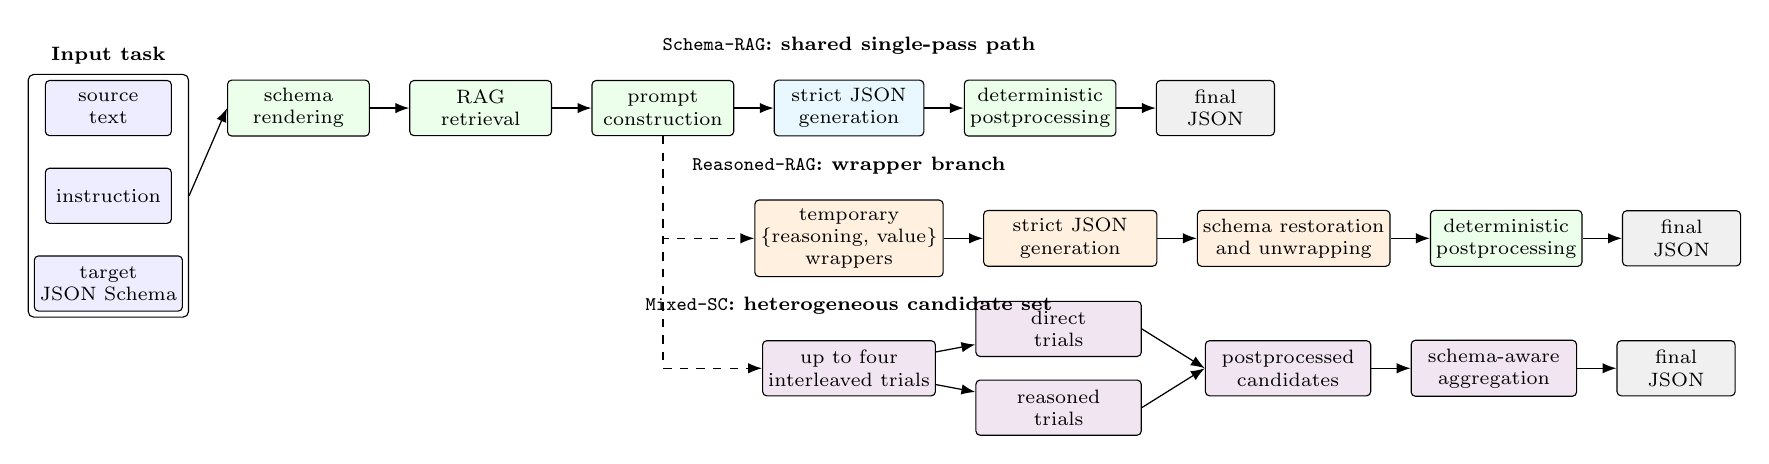
\begin{tikzpicture}[
  font=\scriptsize,
  >=Latex,
  node distance=4mm and 5mm,
  box/.style={draw, rounded corners=1.5pt, align=center, inner xsep=2pt, inner ysep=3pt, minimum height=7mm},
  inputbox/.style={box, fill=blue!7, minimum width=16mm},
  shared/.style={box, fill=green!8, minimum width=18mm},
  direct/.style={box, fill=cyan!9, minimum width=19mm},
  reasoned/.style={box, fill=orange!12, minimum width=22mm},
  mixed/.style={box, fill=violet!10, minimum width=21mm},
  finalbox/.style={box, fill=gray!12, minimum width=15mm},
  groupbox/.style={draw, rounded corners=2pt, inner sep=2pt},
  arrow/.style={->, line width=0.45pt},
  dashedarrow/.style={->, dashed, line width=0.45pt}
]

\node[inputbox] (src) {source\\text};
\node[inputbox, below=of src] (inst) {instruction};
\node[inputbox, below=of inst] (schema) {target\\JSON Schema};
\node[groupbox, fit=(src)(inst)(schema), label={[font=\scriptsize\bfseries]above:Input task}] (input) {};

\node[shared, right=7mm of src] (render) {schema\\rendering};
\node[shared, right=of render] (retrieval) {RAG\\retrieval};
\node[shared, right=of retrieval] (prompt) {prompt\\construction};

\node[direct, right=of prompt] (genD) {strict JSON\\generation};
\node[shared, right=of genD] (postD) {deterministic\\postprocessing};
\node[finalbox, right=of postD] (finalD) {final\\JSON};
\node[font=\scriptsize\bfseries, above=2mm of genD] (schemaLabel) {\texttt{Schema-RAG}: shared single-pass path};

\node[reasoned, below=8mm of genD] (wrapR) {temporary\\\{reasoning, value\}\\wrappers};
\node[reasoned, right=of wrapR] (genR) {strict JSON\\generation};
\node[reasoned, right=of genR] (unwrapR) {schema restoration\\and unwrapping};
\node[shared, right=of unwrapR] (postR) {deterministic\\postprocessing};
\node[finalbox, right=of postR] (finalR) {final\\JSON};
\node[font=\scriptsize\bfseries, above=2mm of wrapR] (reasonLabel) {\texttt{Reasoned-RAG}: wrapper branch};

\node[mixed, below=8mm of wrapR] (trialsM) {up to four\\interleaved trials};
\node[mixed, right=of trialsM, yshift=5mm] (directM) {direct\\trials};
\node[mixed, right=of trialsM, yshift=-5mm] (reasonM) {reasoned\\trials};
\node[mixed, right=8mm of directM, yshift=-5mm] (candM) {postprocessed\\candidates};
\node[mixed, right=of candM] (aggM) {schema-aware\\aggregation};
\node[finalbox, right=of aggM] (finalM) {final\\JSON};
\node[font=\scriptsize\bfseries, above=2mm of trialsM] (mixedLabel) {\texttt{Mixed-SC}: heterogeneous candidate set};

\draw[arrow] (input.east) -- (render.west);
\draw[arrow] (render) -- (retrieval);
\draw[arrow] (retrieval) -- (prompt);
\draw[arrow] (prompt) -- (genD);
\draw[arrow] (genD) -- (postD);
\draw[arrow] (postD) -- (finalD);

\draw[dashedarrow] (prompt.south) |- (wrapR.west);
\draw[arrow] (wrapR) -- (genR);
\draw[arrow] (genR) -- (unwrapR);
\draw[arrow] (unwrapR) -- (postR);
\draw[arrow] (postR) -- (finalR);

\draw[dashedarrow] (prompt.south) |- (trialsM.west);
\draw[arrow] (trialsM) -- (directM);
\draw[arrow] (trialsM) -- (reasonM);
\draw[arrow] (directM.east) -- (candM.west);
\draw[arrow] (reasonM.east) -- (candM.west);
\draw[arrow] (candM) -- (aggM);
\draw[arrow] (aggM) -- (finalM);

\end{tikzpicture}%
}
\caption{Architecture of the submitted DRILLER pipelines. \texttt{Schema-RAG} follows the shared single-pass path, \texttt{Reasoned-RAG} adds temporary reasoning/value wrappers before restoring the original schema, and \texttt{Mixed-SC} aggregates postprocessed candidates from direct and reasoned trials.}
\label{fig:system-architecture}
\end{figure}

The prompt presents the instance instruction, grounding rules, retrieved examples when available, a Pydantic version of the target schema, and the source text. The rules state that the source text is the only evidence, examples are demonstrations rather than facts for the new instance, enum labels must be used exactly, and unsupported nullable fields should be returned as JSON \texttt{null}. This organization keeps the schema and passage close to generation while making the evidence boundary explicit.

Schema rendering has direct and reasoned variants. In direct mode, the JSON Schema is shown as a compact Pydantic-style model: fields become typed attributes, descriptions remain near the fields they define, arrays and nested objects are readable as typed structures, and enums are displayed as literal alternatives. This prompt view is not the formal output contract. The model request also includes a strict JSON Schema response format derived from the target schema, and the final answer is checked against the evaluator-facing schema shape after postprocessing.

Retrieval is also shared. Each extraction can include up to two local few-shot demonstrations selected for schema relevance. Same-schema retrieval is used when examples have the same normalized structural schema as the current task; otherwise, DRILLER falls back to field-level matching over field names, descriptions, type classes, and complementary coverage. The selected examples are rendered in the same output style as the current extractor: direct examples for \texttt{Schema-RAG}, reasoning/value examples for \texttt{Reasoned-RAG}, and trial-specific rendering inside \texttt{Mixed-SC}.

Postprocessing is deterministic and conservative. It parses JSON, cleans common Unicode artifacts, normalizes strings to \textit{Normalization Form C} (NFC), removes temporary reasoning wrappers when present, and converts the literal string \texttt{"null"} to JSON \texttt{null} only at schema positions where null is allowed. It does not infer missing facts, repair unsupported values, or reinterpret the source text after generation.

\texttt{Schema-RAG} is the direct single-pass pipeline. It uses the Pydantic-style prompt schema, retrieves demonstrations, requests a strict JSON object, and returns the parsed and normalized object. Because no reasoning wrapper is used, the generated top-level fields already match the final output interface.

\texttt{Reasoned-RAG} follows the same path but temporarily transforms each top-level field into an object with \texttt{reasoning} and \texttt{value} slots during generation. The prompt schema exposes this as a reasoned value, and the response schema requires the wrapper structure. After generation, DRILLER discards the reasoning strings and returns only the values in the original schema shape.

\texttt{Mixed-SC} moves from a single extraction to a heterogeneous candidate set. It requests up to four budget-aware trials: two direct \texttt{Schema-RAG}-style attempts and two reasoning-augmented \texttt{Reasoned-RAG}-style attempts in an interleaved plan. Each completed trial performs its own retrieval, prompt construction, strict generation, and postprocessing. Aggregation receives final-shape JSON candidates, not raw model messages or reasoning traces, and combines them recursively using schema-aware rules for scalars, nulls, objects, and arrays.

\section{Schema-Guided Prompting}

DRILLER's prompting strategy treats the schema as part of the task semantics, not only as a formatting constraint. The prompt must help the model decide what each field asks for, while the model request must still constrain the response to a JSON object. This section describes the prompt objective, schema rendering, structured response format, and interaction with retrieval and reasoning wrappers.

The prompt objective is to make the model behave as a precise Spanish information extractor. The model is instructed to use the current source text as the only evidence, follow the extraction instruction, and interpret field meanings through the target schema. Retrieved examples are explicitly presented as demonstrations of extraction behavior, not as evidence for the current input. The answer must be only the requested JSON object, without markdown fences, explanations, or extra text.

The standard prompt is organized around the extraction workflow. It first sets the extraction role. It then gives Spanish extraction rules covering grounding, full schema coverage, exact enum labels, conservative null handling, and value normalization when requested by the field description. Retrieved examples are inserted next. Finally, the current schema is rendered in a model-readable form followed by the source text. This order keeps task intent and extraction constraints visible while placing the current schema and evidence near generation.

Raw JSON Schema is well suited for validation, but it can be visually heavy inside a prompt. Nested property dictionaries, separate required lists, repeated keywords, and nullable type arrays can obscure the field descriptions that carry extraction semantics. DRILLER therefore renders the schema in a Pydantic-style view. The view is not an executable program and does not replace the target JSON Schema; it is a compact representation designed to make the current extraction contract easier for the model to read.

In this view, object schemas become class-like structures and properties appear as typed attributes. Primitive fields are rendered as familiar scalar types, arrays as list types, enums as literal alternatives, and nested objects as nested or referenced model types. Nullability is shown near the field rather than separated from the definition. Field descriptions are preserved because they often determine the correct behavior: the same type annotation can require copying, normalization, classification, or a short grounded summary depending on the description.

DRILLER distinguishes three schema roles, summarized in Table~\ref{tab:schema-roles}. The same target schema is transformed differently depending on whether it is being shown to the model, used to constrain decoding, or returned to the evaluator.

\begin{table}[t]
\centering
\small
\caption{Schema roles in DRILLER. The prompt schema supports model comprehension; the generation schema constrains decoding; the final challenge schema defines the returned interface.}
\label{tab:schema-roles}
\begin{tabularx}{\linewidth}{@{}>{\raggedright\arraybackslash}p{0.22\linewidth}
>{\raggedright\arraybackslash}p{0.28\linewidth}
>{\raggedright\arraybackslash}X@{}}
\toprule
Schema role & Where it is used & Function in the system \\
\midrule
Prompt schema &
Text shown inside the extraction prompt &
Pydantic-style or reasoned Pydantic-style rendering that helps the model interpret field names, descriptions, types, enums, nullability, and nesting. \\
Generation schema &
Structured response format sent with the model request &
Strict JSON Schema used to constrain the generated object; in reasoning mode, temporary wrappers are inserted before generation. \\
Final challenge schema &
Shape expected by the evaluator &
Original task schema after postprocessing and optional unwrapping; reasoning scaffolds and prompt-only conventions are not returned. \\
\bottomrule
\end{tabularx}
\end{table}

The prompt schema is a readability layer. It can use class-like declarations, readable nullable notation, and other prompt-only conventions because its purpose is communication. The generation schema has a different role: DRILLER attaches a strict JSON Schema response format to the model request so decoding is constrained toward a JSON object compatible with the requested structure.

For the submitted non-baseline pipelines, declared object properties are required during generation. This reduces field omissions, a common failure mode when a model understands the task but leaves out keys. Requiring keys does not require every value to be substantive. If the target schema permits null, the generated object may include the key with JSON \texttt{null}. The final challenge schema remains the original schema shape; generation-time requiredness is an inference constraint, not permission to fabricate unsupported content.

Reasoning wrappers create a second schema variant. In direct mode, used by \texttt{Schema-RAG}, the prompt schema is ordinary Pydantic-style rendering and the model produces final values directly. In reasoning mode, used by \texttt{Reasoned-RAG} and the reasoning-augmented trials of \texttt{Mixed-SC}, each top-level field is shown as a reasoned value. The temporary generation schema requires an object with \texttt{reasoning} and \texttt{value} fields for each top-level slot. The \texttt{value} field retains the original type, including enums, arrays, objects, and nullable alternatives.

This transformation is a schema-guided interface change rather than a request for free-form explanation. The model has a structured place to state local evidence or absence before committing to a field value, but the reasoning text is removed during postprocessing. Direct and reasoned prompting therefore share the same final objective while exposing different intermediate interfaces.

Prompting also interacts with retrieval. In the general RAG layout, each example carries enough schema context for the model to understand why its output follows from its own source text and schema. In the same-schema layout, selected examples share the normalized target schema, so DRILLER can render the shared schema once and show compact example inputs and outputs. This saves prompt size and lets the examples emphasize contrasting field outcomes under the same structure.

Examples can show how fields are populated, when null or empty arrays are appropriate, and how enum labels or nested structures behave, but their values are not evidence for the current instance. In reasoning mode, retrieved examples are rendered with the same temporary \texttt{\{reasoning, value\}} structure expected from the current extractor; in direct mode, examples use final field values. \texttt{Mixed-SC} applies the appropriate layout separately inside each trial.

Overall, schema-guided prompting in DRILLER combines readable schema presentation, explicit grounded-extraction rules, strict structured generation, and retrieval-aware layout. The purpose is to make schema interpretation explicit while returning a complete JSON object compatible with the evaluator-facing schema.

\section{Field-Aware Few-Shot Retrieval}

DRILLER retrieves examples for schema interpretation. In a variable-schema task, semantic similarity between source texts is not enough: two passages may be topically close but ask for different fields, while two different domains may instantiate similar extraction behavior. The submitted pipelines retrieve demonstrations using schema structure, extraction instruction, field descriptions, type compatibility, and complementary output behavior. \texttt{Schema-RAG}, \texttt{Reasoned-RAG}, and every trial of \texttt{Mixed-SC} use the same retrieval path.

Figure~\ref{fig:retrieval-map} summarizes the two retrieval paths used by DRILLER.

\definecolor{drillfigblue}{RGB}{59,89,119}
\definecolor{drillfigteal}{RGB}{72,112,105}
\definecolor{drillfiggold}{RGB}{150,124,62}
\definecolor{drillfigline}{RGB}{88,88,88}

\begin{figure}[t]
\centering
\resizebox{\linewidth}{!}{%
\begin{tikzpicture}[
  font=\scriptsize,
  >=Latex,
  line cap=round,
  line join=round,
  panel/.style={
    draw=black!34,
    fill=black!2,
    rounded corners=3pt,
    line width=0.45pt
  },
  subpanel/.style={
    draw=black!28,
    fill=white,
    rounded corners=2.4pt,
    line width=0.36pt
  },
  card/.style={
    draw=black!46,
    fill=white,
    rounded corners=2pt,
    line width=0.42pt
  },
  querypart/.style={
    draw=black!25,
    fill=black!3,
    rounded corners=1.5pt,
    line width=0.32pt,
    inner sep=2.1pt,
    align=left,
    font=\tiny
  },
  badge/.style={
    draw=black!42,
    fill=white,
    rounded corners=2pt,
    line width=0.34pt,
    inner xsep=2.5pt,
    inner ysep=1.2pt,
    font=\scriptsize\bfseries
  },
  chip/.style={
    draw=black!35,
    fill=black!5,
    rounded corners=2pt,
    line width=0.30pt,
    inner xsep=2.0pt,
    inner ysep=0.9pt,
    font=\tiny
  },
  route/.style={
    -{Latex[length=2.0mm]},
    draw=drillfigline,
    line width=0.66pt
  },
  express/.style={
    -{Latex[length=2.1mm]},
    draw=drillfigblue,
    line width=1.05pt
  },
  fallback/.style={
    -{Latex[length=2.0mm]},
    draw=drillfigteal,
    line width=0.84pt,
    densely dashed
  },
  selected/.style={
    card,
    draw=drillfigblue!85!black,
    fill=drillfigblue!6,
    line width=0.82pt
  },
  selectedfallback/.style={
    card,
    draw=drillfigteal!80!black,
    fill=drillfigteal!6,
    line width=0.82pt
  },
  promptitem/.style={
    draw=black!32,
    fill=black!3,
    rounded corners=1.2pt,
    line width=0.26pt,
    inner xsep=0.85pt,
    inner ysep=0.55pt,
    outer sep=0pt,
    font=\tiny,
    align=center
  }
]

% Main grouping panels.
\node[panel, minimum width=2.62cm, minimum height=6.16cm, anchor=south west] (querypanel) at (0.05,0.62) {};
\node[panel, minimum width=6.78cm, minimum height=2.48cm, anchor=south west, fill=drillfigblue!4] (upperpanel) at (3.05,4.33) {};
\node[panel, minimum width=6.78cm, minimum height=3.28cm, anchor=south west, fill=drillfigteal!4] (lowerpanel) at (3.05,0.62) {};
\node[panel, minimum width=2.58cm, minimum height=6.16cm, anchor=south west] (selectedpanel) at (10.10,0.62) {};
\node[panel, minimum width=3.07cm, minimum height=6.16cm, anchor=south west] (promptpanel) at (12.68,0.62) {};

\node[badge, fill=black!4, anchor=west, inner xsep=1.6pt] at (0.24,6.55) {Query instance \(q\)};
\node[badge, draw=drillfigblue!60!black, fill=drillfigblue!8, anchor=west] at (3.24,6.56) {same-schema retrieval};
\node[chip, draw=drillfigblue!65!black, fill=white, anchor=east] at (9.62,6.55) {FAST PATH};
\node[badge, draw=drillfigteal!65!black, fill=drillfigteal!8, anchor=west] at (3.24,3.65) {field-level fallback};
\node[chip, draw=drillfigteal!65!black, fill=white, anchor=east] at (9.62,3.64) {ANALYTICAL};
\node[badge, fill=black!4, anchor=west] at (10.25,6.55) {Retrieved};
\node[badge, fill=black!4, anchor=west] at (12.83,6.55) {Prompt integration};

% Query card.
\node[card, minimum width=2.12cm, minimum height=5.22cm, anchor=north west] (querycard) at (0.36,6.23) {};
\draw[draw=black!34, fill=black!10, line width=0.32pt]
  (2.19,6.23) -- (2.48,6.23) -- (2.48,5.94) -- cycle;
\draw[draw=black!28, line width=0.32pt] (2.19,6.23) -- (2.48,5.94);
\node[querypart, text width=1.62cm, anchor=north west] at (0.53,5.88)
  {\textbf{instruction}\\extract fields};
\node[querypart, text width=1.62cm, anchor=north west] at (0.53,4.90)
  {\textbf{source text}\\short passage};
\node[querypart, text width=1.62cm, anchor=north west] at (0.53,3.92)
  {\textbf{target JSON Schema}\\types, enums, req.};
\node[font=\tiny\bfseries, text=black!65, anchor=west] at (0.53,2.69) {extracted views};
\node[chip, draw=drillfigblue!55!black, fill=drillfigblue!7, anchor=west] at (0.53,2.36) {\(\phi(S_q)\)};
\node[chip, draw=drillfigteal!60!black, fill=drillfigteal!7, anchor=west] at (0.53,2.05) {\(f_1,\ldots,f_m\)};
\node[font=\tiny, text=black!60, align=center, text width=1.72cm] at (1.38,1.58)
  {schema identity\\and field list};

% Same-schema lane.
\coordinate (qout) at (2.67,5.48);
\draw[route] (2.48,5.48) -- (qout);
\draw[express] (qout) -- (3.12,5.48);

\node[font=\tiny\bfseries, text=black!70, anchor=west] at (3.24,6.12) {FSP candidates};
\foreach \x/\lab/\shade in {3.32/\(c_1\)/4,3.69/\(c_2\)/9,4.06/\(c_3\)/4,4.35/\(\cdots\)/11} {
  \node[card, fill=black!\shade, minimum width=0.38cm, minimum height=0.68cm] at (\x,5.48) {};
  \node[font=\tiny] at (\x,5.48) {\lab};
}
\draw[express] (4.54,5.48) -- (4.98,5.48);
\node[card, draw=drillfigblue!65!black, fill=white, minimum width=0.95cm, minimum height=1.18cm, align=center, font=\scriptsize] (gate) at (5.52,5.48)
  {\(\phi(S_q)\)\\[-1pt]\(=\phi(S_c)\)};
\node[font=\tiny, text=black!62] at (5.52,4.75) {hard filter};
\draw[express] (6.01,5.48) -- (6.40,5.48);

\node[card, minimum width=1.50cm, minimum height=1.22cm] (rankbox) at (7.17,5.48) {};
\node[font=\tiny\bfseries, align=center] at (7.17,5.90) {semantic\\rank};
\node[font=\tiny] at (7.17,5.58) {\(\operatorname{sim}(r_q,r_c)\)};
\draw[fill=drillfigblue!55, draw=black!20, line width=0.22pt] (6.62,5.34) rectangle (7.48,5.43);
\draw[fill=drillfigblue!35, draw=black!20, line width=0.22pt] (6.62,5.16) rectangle (7.28,5.25);
\draw[fill=black!22, draw=black!20, line width=0.22pt] (6.62,4.98) rectangle (7.02,5.07);
\draw[express] (7.91,5.48) -- (8.24,5.48);

% Explicit same-schema decision node.
\coordinate (dec) at (8.76,5.48);
\draw[draw=drillfigblue!70!black, fill=white, line width=0.55pt]
  (8.76,5.98) -- (9.28,5.48) -- (8.76,4.98) -- (8.24,5.48) -- cycle;
\node[font=\tiny\bfseries, align=center] at (8.76,5.55) {\(\geq 2\)\\pass \(\tau\)?};
\node[font=\tiny, text=drillfigblue!70!black, anchor=south] at (9.46,5.62) {YES};
\draw[express] (9.28,5.48) -- (10.10,5.48);

% Fallback control flow from the decision.
\node[font=\tiny, text=drillfigteal!75!black, align=center, text width=0.88cm, anchor=north] at (9.38,5.16)
  {NO:\\field-level\\fallback};
\draw[fallback] (8.76,4.98) -- (8.76,4.18) -- (3.36,4.18) -- (3.36,3.90);

% Field-level fallback lane.
\node[font=\tiny\bfseries, text=black!70, anchor=west] at (3.34,3.28) {type-compatible field similarity};
\foreach \x/\lab in {3.86/\(c_1\),4.24/\(c_2\),4.62/\(c_3\),5.00/\(\cdots\)} {
  \node[font=\tiny] at (\x,3.02) {\lab};
}
\foreach \y/\lab in {2.72/\(f_1\),2.42/\(f_2\),2.12/\(f_3\),1.82/\(f_m\)} {
  \node[font=\tiny, anchor=east] at (3.62,\y) {\lab};
}
\foreach \x/\y/\shade in {
  3.70/2.58/65,4.08/2.58/28,4.46/2.58/12,4.84/2.58/45,
  3.70/2.28/18,4.08/2.28/62,4.46/2.28/34,4.84/2.28/10,
  3.70/1.98/48,4.08/1.98/14,4.46/1.98/58,4.84/1.98/22,
  3.70/1.68/10,4.08/1.68/42,4.46/1.68/26,4.84/1.68/60
} {
  \draw[draw=black!18, fill=black!\shade, line width=0.23pt] (\x,\y) rectangle ++(0.30,0.26);
}
\draw[draw=black!40, line width=0.32pt] (3.70,1.68) rectangle (5.14,2.84);
\draw[draw=drillfigteal!78!black, line width=0.58pt, rounded corners=1pt] (3.67,1.64) rectangle (4.03,2.88);
\draw[draw=drillfigteal!78!black, line width=0.58pt, rounded corners=1pt, densely dashed] (4.05,1.64) rectangle (4.41,2.88);
\node[chip, draw=drillfigteal!60!black, fill=white, font=\tiny] at (4.42,1.23)
  {\(\kappa(f_i)\sim\kappa(g)\)};
% Field-similarity vectors tied to selected heatmap columns.
\draw[fallback, line width=0.58pt] (4.03,2.64) -- (5.50,2.42);
\draw[fallback, line width=0.58pt] (4.41,2.24) -- (5.50,1.52);
\node[font=\tiny, anchor=south] at (6.02,2.82) {\(v(c_1)\)};
\node[card, minimum width=1.05cm, minimum height=0.72cm] (vonebox) at (6.02,2.38) {};
\draw[fill=drillfigteal!55, draw=black!20, line width=0.2pt] (5.70,2.14) rectangle ++(0.10,0.32);
\draw[fill=drillfigteal!25, draw=black!20, line width=0.2pt] (5.88,2.14) rectangle ++(0.10,0.15);
\draw[fill=drillfigteal!45, draw=black!20, line width=0.2pt] (6.06,2.14) rectangle ++(0.10,0.27);
\draw[fill=black!20, draw=black!20, line width=0.2pt] (6.24,2.14) rectangle ++(0.10,0.10);

\node[card, minimum width=1.05cm, minimum height=0.72cm] (vtwobox) at (6.02,1.50) {};
\draw[fill=drillfigteal!25, draw=black!20, line width=0.2pt] (5.70,1.26) rectangle ++(0.10,0.13);
\draw[fill=drillfigteal!55, draw=black!20, line width=0.2pt] (5.88,1.26) rectangle ++(0.10,0.34);
\draw[fill=black!20, draw=black!20, line width=0.2pt] (6.06,1.26) rectangle ++(0.10,0.11);
\draw[fill=drillfigteal!48, draw=black!20, line width=0.2pt] (6.24,1.26) rectangle ++(0.10,0.28);
\node[font=\tiny, anchor=north] at (6.02,1.05) {\(v(c_2)\)};

\draw[fallback] (6.58,2.02) -- (6.82,2.02);
\node[card, minimum width=1.78cm, minimum height=0.88cm, align=center, font=\tiny] (objective) at (8.05,2.80)
  {\(s(c_1,c_2)=\)\\[-1pt]
   \(\|v(c_1)+v(c_2)\|_2\)\\[-1pt]
   \(+\|v(c_1)-v(c_2)\|_2\)};
\node[card, minimum width=1.36cm, minimum height=0.80cm] (joint) at (7.35,1.48) {};
\node[font=\tiny\bfseries] at (7.35,1.78) {coverage};
\node[font=\tiny] at (7.35,1.58) {\(v_1+v_2\)};
\draw[fill=drillfiggold!55, draw=black!20, line width=0.2pt] (6.92,1.15) rectangle ++(0.14,0.22);
\draw[fill=drillfiggold!50, draw=black!20, line width=0.2pt] (7.15,1.15) rectangle ++(0.14,0.31);
\draw[fill=drillfiggold!38, draw=black!20, line width=0.2pt] (7.38,1.15) rectangle ++(0.14,0.25);
\draw[fill=drillfiggold!48, draw=black!20, line width=0.2pt] (7.61,1.15) rectangle ++(0.14,0.28);
\node[card, minimum width=1.50cm, minimum height=0.80cm] (diff) at (8.85,1.48) {};
\node[font=\tiny\bfseries] at (8.85,1.78) {complement};
\node[font=\tiny] at (8.85,1.58) {\(v_1-v_2\)};
\draw[draw=black!38, line width=0.25pt] (8.35,1.28) -- (9.36,1.28);
\draw[fill=drillfigteal!45, draw=black!20, line width=0.2pt] (8.40,1.28) rectangle ++(0.16,0.17);
\draw[fill=drillfigteal!30, draw=black!20, line width=0.2pt] (8.68,1.16) rectangle ++(0.16,0.12);
\draw[fill=drillfigteal!42, draw=black!20, line width=0.2pt] (8.96,1.28) rectangle ++(0.16,0.14);
\draw[fill=drillfigteal!35, draw=black!20, line width=0.2pt] (9.24,1.14) rectangle ++(0.16,0.14);
\draw[fallback] (9.52,2.20) -- (10.10,2.20);

% Selected demonstrations panel, split by retrieval mode.
\node[subpanel, minimum width=2.26cm, minimum height=2.51cm, anchor=south west] (sameselpanel) at (10.26,3.82) {};
\node[subpanel, minimum width=2.26cm, minimum height=2.62cm, anchor=south west] (fbselpanel) at (10.26,0.88) {};
\node[font=\tiny\bfseries, anchor=west] at (10.38,6.10) {same-schema outputs};
\node[font=\tiny, text=black!62, anchor=west] at (10.38,5.87) {shared schema};
\node[selected, text width=0.72cm, minimum height=0.70cm, align=center, font=\tiny] at (10.82,5.42)
  {\textbf{Ex. 1}\\demo};
\node[selected, text width=0.72cm, minimum height=0.70cm, align=center, font=\tiny] at (11.72,5.42)
  {\textbf{Ex. 2}\\demo};
\draw[draw=drillfigblue!65!black, line width=0.45pt] (10.50,5.05) -- (12.05,5.05);
\node[chip, draw=drillfigblue!55!black, fill=white] at (11.26,4.78) {null vs grounded};
\node[chip, draw=drillfigblue!55!black, fill=white] at (11.26,4.50) {empty vs populated};
\node[chip, draw=drillfigblue!55!black, fill=white] at (11.26,4.22) {enum contrast};

\node[font=\tiny\bfseries, anchor=west] at (10.38,3.34) {fallback outputs};
\node[font=\tiny, text=black!62, anchor=north west, align=left, text width=1.36cm, inner sep=0pt] at (10.38,3.15) {complementary\\[-1pt]coverage};
\node[selectedfallback, text width=1.74cm, minimum height=0.82cm, align=left, font=\tiny] at (11.39,2.24)
  {\textbf{Ex. 1}\hfill \(f_1\ f_3\)};
\draw[fill=drillfigteal!55, draw=black!20, line width=0.18pt] (10.62,1.90) rectangle ++(0.20,0.22);
\draw[fill=black!15, draw=black!20, line width=0.18pt] (10.91,1.90) rectangle ++(0.20,0.08);
\draw[fill=drillfigteal!48, draw=black!20, line width=0.18pt] (11.20,1.90) rectangle ++(0.20,0.19);
\draw[fill=black!15, draw=black!20, line width=0.18pt] (11.49,1.90) rectangle ++(0.20,0.07);
\node[selectedfallback, text width=1.74cm, minimum height=0.82cm, align=left, font=\tiny] at (11.39,1.36)
  {\textbf{Ex. 2}\hfill \(f_2\ f_m\)};
\draw[fill=black!15, draw=black!20, line width=0.18pt] (10.62,1.02) rectangle ++(0.20,0.08);
\draw[fill=drillfigteal!56, draw=black!20, line width=0.18pt] (10.91,1.02) rectangle ++(0.20,0.24);
\draw[fill=black!15, draw=black!20, line width=0.18pt] (11.20,1.02) rectangle ++(0.20,0.08);
\draw[fill=drillfigteal!48, draw=black!20, line width=0.18pt] (11.49,1.02) rectangle ++(0.20,0.20);
% Prompt integration panel, split by rendering layout.
\node[subpanel, minimum width=2.86cm, minimum height=2.23cm, anchor=south west] (samepromptpanel) at (12.78,4.10) {};
\node[subpanel, minimum width=2.86cm, minimum height=2.92cm, anchor=south west] (ragpromptpanel) at (12.78,0.88) {};
\node[font=\tiny\bfseries, anchor=west] at (12.90,6.13) {same-schema assembly};
\node[promptitem, minimum width=0.80cm, minimum height=0.22cm, fill=black!3] at (13.94,5.84) {rules};
\node[promptitem, minimum width=1.16cm, minimum height=0.22cm, fill=drillfigblue!7] at (14.84,5.84) {schema \(S_q\)};
\foreach \y/\lab in {5.38/Ex. 1,5.00/Ex. 2} {
  \node[font=\tiny\bfseries, anchor=east] at (13.64,\y) {\lab};
  \node[promptitem, minimum width=0.48cm, minimum height=0.22cm] at (13.96,\y) {instr};
  \node[promptitem, minimum width=0.44cm, minimum height=0.22cm] at (14.54,\y) {src};
  \node[promptitem, minimum width=0.44cm, minimum height=0.22cm] at (15.10,\y) {out};
  \draw[draw=black!38, -{Latex[length=0.8mm]}, line width=0.24pt] (14.24,\y) -- (14.30,\y);
  \draw[draw=black!38, -{Latex[length=0.8mm]}, line width=0.24pt] (14.82,\y) -- (14.88,\y);
}
\node[font=\tiny\bfseries, anchor=east] at (13.72,4.62) {current};
\node[promptitem, minimum width=0.48cm, minimum height=0.22cm, fill=drillfigblue!5] at (13.96,4.62) {instr};
\node[promptitem, minimum width=0.44cm, minimum height=0.22cm, fill=drillfigblue!5] at (14.54,4.62) {src};
\draw[draw=black!38, -{Latex[length=0.8mm]}, line width=0.24pt] (14.24,4.62) -- (14.30,4.62);

\node[font=\tiny\bfseries, anchor=west] at (12.90,3.57) {general RAG assembly};
\foreach \y/\lab/\schema in {3.08/Ex. 1/\(S_{c_1}\),2.32/Ex. 2/\(S_{c_2}\)} {
  \node[promptitem, minimum width=1.72cm, minimum height=0.56cm] at (14.56,\y) {};
  \node[font=\tiny\bfseries, anchor=east] at (13.56,\y+0.16) {\lab};
  \node[promptitem, minimum width=0.48cm, minimum height=0.18cm] at (14.06,\y+0.16) {instr};
  \node[promptitem, minimum width=0.62cm, minimum height=0.18cm, fill=drillfigteal!7] at (14.80,\y+0.16) {\schema};
  \node[promptitem, minimum width=0.46cm, minimum height=0.18cm] at (14.06,\y-0.15) {src};
  \node[promptitem, minimum width=0.46cm, minimum height=0.18cm] at (14.80,\y-0.15) {out};
  \draw[draw=black!38, -{Latex[length=0.8mm]}, line width=0.24pt] (14.34,\y-0.15) -- (14.50,\y-0.15);
}
\node[promptitem, minimum width=1.72cm, minimum height=0.48cm, fill=drillfigteal!6] at (14.56,1.52) {};
\node[font=\tiny\bfseries, anchor=east] at (13.72,1.64) {current};
\node[promptitem, minimum width=0.48cm, minimum height=0.18cm, fill=white] at (14.06,1.64) {instr};
\node[promptitem, minimum width=0.62cm, minimum height=0.18cm, fill=white] at (14.80,1.64) {\(S_q\)};
\node[promptitem, minimum width=0.46cm, minimum height=0.18cm, fill=white] at (14.44,1.32) {src};

% Mode-specific integration arrows.
\draw[express] (12.52,5.48) -- (12.82,5.48);
\draw[fallback] (12.52,2.20) -- (12.82,2.20);

\end{tikzpicture}%
}
\caption{Two-stage retrieval in DRILLER. The system first attempts same-schema retrieval by filtering candidate demonstrations with a normalized schema fingerprint and ranking surviving cases semantically. A decision node routes directly to same-schema demonstrations when at least two cases pass the threshold; otherwise, field-level fallback scores candidates by type-compatible field similarity and selects a complementary pair. The selected demonstrations are then rendered with either the compact same-schema prompt layout or the general RAG layout.}
\label{fig:retrieval-map}
\end{figure}


\subsection{Curated Demonstration Corpus}

The retrieval pool is a local few-shot prompting (FSP) corpus of structured extraction demonstrations. Each case contains a Spanish source text, an extraction instruction, a target schema, expected values, tags describing covered extraction phenomena, and field-level rationales or descriptions that support rendering examples in either direct or reasoning-augmented form. The corpus is synthetic and curated rather than mined from an external collection.

The GenSIE development set guided corpus design. We used it to study schema structure, source-text style, vocabulary, noise patterns, and recurring ambiguities, rather than reusing development instances as demonstrations. We also manually curated a small development-time evaluation subset, reviewing up to two instances per task family. Those curated instances served as design references only. Direct reuse would not provide systematic complementary coverage of field dualities and would contaminate evaluation on the same curated subset, since retrieval could return the instance being solved.

We constructed the final FSP corpus as a compact library of synthetic and manually curated structured cases, organized by development task family and schema family. The corpus used an author-in-the-loop workflow assisted by an agentic LLM coding assistant. The assistant helped inspect candidate task families, draft complementary-case proposals, generate provisional source texts and structured resources, and run structural checks. The authors reviewed and corrected the proposed dualities, source texts, expected outputs, reasoning fields, enriched descriptions, and final JSON resources before inclusion. The workflow was:

\begin{enumerate}
\item Each development task family became the unit of work because a family bundles a schema, domain, source-text style, vocabulary, and recurring extraction traps.
\item The assistant inspected the curated development subset first, then consulted the full uncurated development set when more evidence about style, structure, or ambiguity was needed. The full set characterized text length, noise patterns, and extraction behavior, but was not treated as trusted gold output.
\item The assistant identified useful field-level dualities: nullable value versus grounded non-null value; empty array versus populated array; boolean \texttt{true} versus \texttt{false}; frequent enum label versus an alternative label; direct or near-verbatim text versus grounded summary; explicit value versus distractor or insufficient evidence; and normalized value versus literal mention.
\item It then proposed two complementary cases for the task or schema family, using a balanced or approximately balanced mask over dual fields as a design heuristic. One case covered one side of several dualities and the second covered the inverse side; qualitative contrasts such as enum A versus enum B or explicit date versus nearby distractor date were handled outside a rigid binary mask.
\item The authors reviewed this pre-drafting proposal, including selected references, field dualities, complementary mask, and intended case behavior. Full synthetic drafting began only after this gate was accepted.
\item Under the approved design, the assistant drafted synthetic Spanish source texts, candidate expected outputs, and field-level reasoning. The texts had to ground values, \texttt{null}s, and empty arrays naturally, resemble the reviewed family style, and avoid benchmark-aware phrases that mechanically announced the expected answer or absence.
\item The authors manually curated the drafted cases before final resource generation, editing source texts, expected outputs, and field-level reasoning. This review checked that each value, \texttt{null}, and empty list was justified by the source text and that the pair contrasted the intended regimes.
\item After author approval, the assistant generated the final \texttt{StructuredFspCase} JSON resources, including \texttt{field\_examples}, tags, field-level reasoning, and enriched descriptions when applicable. The resources were loaded through the FSP resource loader or equivalent structural checks before retrieval used them.
\end{enumerate}

The final extraction corpus contains two cases for each of the 22 schema or task families represented in the curated development setting, for 44 extraction cases in the local retrieval pool. The families cover a range of domains and structures, but the corpus is not intended to be a large topical nearest-neighbor database. It is a compact library of contrasted demonstrations: the useful unit is often a pair of cases showing how the same or related fields behave under different evidence conditions.

The paired organization is deliberate. A nullable field benefits from both grounded non-null values and grounded absence. An array field benefits from examples where the correct list is populated and examples where it is empty. Enum fields benefit from contrasting labels, especially when labels are inferred rather than copied literally. Numeric and date fields may require exact copying in one case and normalization in another. String fields may require direct mention extraction, near-verbatim evidence, or a short grounded summary depending on the field description.

After complementary cases had been proposed and reviewed, we added enriched field descriptions as compact Spanish prompt annotations. They explain how to extract a field and warn about traps observed during development-example review or synthetic case construction, such as distractor dates, nearby but semantically wrong entities, aliases, or conditions under which a nullable field should remain \texttt{null}. These descriptions clarify schema semantics for same-schema prompting; they do not add new instance evidence. They appear only in the prompt-side schema view. The target JSON Schema, strict generation schema, and evaluator-facing output schema remain unchanged.

The FSP reasoning fields follow the structured evidence discipline. In reasoning-mode examples, each field can render \texttt{field\_asks}, \texttt{relevant\_fragments}, and \texttt{final\_value} as a local evidence protocol. Cited fragments support the extraction decision rather than merely repeating the answer string. They stay short while preserving the context needed to justify the value: accepted candidates show why the value belongs to the requested field, and rejected or \texttt{null} cases cite the closest reviewed context and state which required assertion is missing. Enum reasoning considers the allowed labels and justifies the selected label from relevant fragments. Array reasoning may cite a complete list once, or cite compactly around individual items, so examples support recall without bloating the prompt. FSP examples therefore demonstrate grounding behavior as well as output formatting.

Table~\ref{tab:technical-software-fsp-pair} gives one compact example from the \texttt{technical\_software} family. The two cases share the same schema but expose complementary regimes: one case grounds populated arrays and leaves several adversarial nullable fields unsupported, while the other inverts the pattern with empty arrays, alias resolution, exact date normalization, an explicit stable-installer checksum, and explicit corporate metadata.

\begin{table}[t]
\centering
\footnotesize
\setlength{\tabcolsep}{3pt}
\caption{Complementary FSP pair for the \texttt{technical\_software} schema family.}
\label{tab:technical-software-fsp-pair}
\begin{tabularx}{\linewidth}{@{}>{\raggedright\arraybackslash}p{0.20\linewidth}
>{\raggedright\arraybackslash}X
>{\raggedright\arraybackslash}X@{}}
\toprule
Field or contrast & \textit{Lince Editor} case & \textit{QuantaPack Pro} case \\
\midrule
\texttt{official\_name} and \texttt{app\_category} &
Direct product name; enum maps to \texttt{IDE\_EDITOR}. &
Abbreviated heading must resolve to full name; enum maps to \texttt{ARCHIVER}. \\
\texttt{platforms} and \texttt{features} &
Populated arrays with named operating systems and technical capabilities. &
Empty arrays: installers and downloads are mentioned, but no supported OS or concrete feature list. \\
\texttt{exact\_release\_date} &
\texttt{null}: only year-level or relative release evidence is present. &
Exact first-release date normalized to \texttt{DD/MM/YYYY}. \\
\path{latest_stable_version_sha256} &
\texttt{null}: PGP signatures and a nightly commit hash are distractors. &
Explicit SHA256 for the stable installer. \\
\texttt{current\_ceo\_name} &
\texttt{null}: founder, idea author, and coordinating team are not CEO evidence. &
Explicit current CEO of the developing company. \\
Pair lesson &
Extract grounded scalar values and populated arrays, but abstain for nullable fields with only distractor evidence. &
Resolve aliases, keep unsupported arrays empty, and fill nullable fields only when the source states the required evidence. \\
\bottomrule
\end{tabularx}
\end{table}

Coverage includes null versus non-null values, present versus absent evidence, enum alternatives, empty versus populated arrays, arrays of simple values, arrays of objects, nested objects, direct strings, summary strings, boolean inference, numeric normalization, date normalization, bounded scores, long evidence spans, and distractor mentions. These contrasts matter because few-shot examples can bias the model when they show only one outcome regime. Complementary demonstrations teach conditional behavior: extract when evidence exists, abstain when it does not, normalize only when requested, and respect the requested type and label set.

\subsection{Same-Schema Retrieval}

At runtime, DRILLER first tries to retrieve examples with the same normalized schema as the current task. Let \(S_q\) be the target schema of query instance \(q\), and let \(S_c\) be the schema of a candidate case \(c\). DRILLER computes a normalized schema fingerprint \(\phi(S)\) by canonicalizing the JSON representation while preserving the structural extraction contract: field names, object structure, array structure, primitive types, enum alternatives, required properties, and nesting. Descriptions are neutralized so that prompt wording refinements do not change schema identity. Order-insensitive elements such as \texttt{required}, \texttt{enum}, and array-valued \texttt{type} are sorted before serialization. Same-schema candidates satisfy the hard constraint
\[
\phi(S_q)=\phi(S_c).
\]

The fingerprint separates schema identity from topical similarity. A medical passage and a technical passage might both contain names, dates, arrays, and classifications without sharing an extraction form. Conversely, two source texts from the same schema family may require the same field interpretation even when their values differ. Same-schema retrieval therefore treats structural identity as a filter rather than as a soft ranking feature.

Filtered candidates are then ranked semantically. DRILLER builds a global textual representation \(r(q)\) of the current task from the task identifier, extraction instruction, and textual representations of top-level fields. Candidate cases are represented analogously as \(r(c)\). These representations are embedded and compared by cosine similarity,
\[
\operatorname{sim}(r(q),r(c)).
\]
The submitted system uses a same-schema threshold \(\tau=0.6\). If at least two fingerprint-matching candidates satisfy \(\operatorname{sim}(r(q),r(c))\geq\tau\), DRILLER selects the top candidates by similarity and marks them as same-schema demonstrations. If fewer than two candidates pass this test, retrieval continues with the field-level fallback.

Same-schema examples show the exact output contract under different source texts. They clarify what counts as evidence for a field, when null or an empty list is correct, and how enum labels or nested structures are populated. They also enable a compact prompt layout: the shared schema is rendered once, and examples focus on instruction, source text, and expected output rather than repeating identical schema blocks.

Same-schema mode can also enrich the prompt-side schema view with curated field descriptions drawn from the selected cases. These enriched descriptions add task and domain guidance such as enum interpretation, null traps, or distractor patterns to the schema text shown to the model. They do not modify the target JSON Schema, the strict generation schema, or the final evaluator-facing schema.

\subsection{Field-Level Retrieval Fallback}

When same-schema retrieval does not produce enough candidates, DRILLER falls back to field-level retrieval. Let the query top-level fields be \(F_q=\{f_1,\ldots,f_m\}\), in schema order, and let \(F_c\) be the top-level fields of candidate case \(c\). Each field \(f\) is mapped to a textual representation \(t(f)\) that combines its field name, readable type, and description, for example ``\texttt{name (type): description}''. The retriever also assigns a coarse type class \(\kappa(f)\), ignoring nullability.

The coarse classes used by the retriever are \texttt{string}, \texttt{boolean}, \texttt{numeric} for both integer and number fields, \texttt{enum}, \texttt{object}, and recursively typed arrays such as \texttt{array[string]}, \texttt{array[numeric]}, \texttt{array[enum]}, and \texttt{array[object]}. A fallback \texttt{any} class is available for unsupported or underspecified schemas. We write \(\kappa(f_i)\sim\kappa(g)\) for compatibility; in the submitted implementation this relation is equality of the nullability-insensitive coarse classes. Thus nullable and non-nullable variants of the same base type can match, while an array of objects is not aligned with a scalar summary merely because their descriptions share topical words.

For each candidate \(c\), DRILLER embeds the field texts \(e(t(f))\) and computes, for every query field \(f_i\), the best compatible field match in the candidate:
\[
a_i(c)=
\max\left(0,\max_{g\in F_c,\ \kappa(g)\sim\kappa(f_i)}
\cos(e(t(f_i)),e(t(g)))\right),
\]
with \(a_i(c)=0\) when no compatible candidate field exists. The candidate is therefore represented by a field-similarity vector aligned with the current query schema,
\[
v(c)=(a_1(c),\ldots,a_m(c)).
\]
A candidate's individual relevance can be summarized by \(\lVert v(c)\rVert_2\), but two-example selection uses a pair-level objective over these same vectors.

The type-aware vector prevents topical retrieval from ignoring output shape. It avoids matching semantically similar descriptions with incompatible JSON structures, allows nullable and non-nullable variants of the same base type to reinforce each other, and shows whether a candidate is broadly useful or strong for only part of the schema. Since retrieval selects a pair of demonstrations, two individually imperfect candidates can be preferable when they cover different field behaviors.

If embedding retrieval fails or produces no usable candidates, DRILLER uses a lexical/schema fallback. It scores candidates with explicit features such as exact normalized schema matches, compatible field fingerprints, tag overlap, field-name overlap, shared terms, and domain-term overlap, with a small penalty for long example texts. This fallback preserves schema-aware retrieval when embeddings are unavailable or uninformative.

\subsection{Complementary Pair Selection}

The submitted RAG path retrieves up to two examples. In the field-level fallback, DRILLER selects a pair with a complementarity-aware objective rather than choosing the two highest individual scores. For two candidate demonstrations \(c_1\) and \(c_2\), with field-similarity vectors \(v(c_1)\) and \(v(c_2)\) defined above, the pair score is

\[
s(c_1,c_2) = \lVert v(c_1)+v(c_2)\rVert_2 + \lVert v(c_1)-v(c_2)\rVert_2 .
\]

The first term, \(\lVert v(c_1)+v(c_2)\rVert_2\), rewards joint relevance and field coverage. If both examples provide useful analogues for the current schema, their combined vector has large magnitude. This term aligns with the ordinary retrieval goal that demonstrations should be relevant to the task.

The second term, \(\lVert v(c_1)-v(c_2)\rVert_2\), rewards complementarity. If two candidates are strong on the same fields and weak on the same fields, their difference vector is small. If one is strong where the other is weak, the difference grows. This discourages near-duplicate demonstrations that reinforce one behavior while leaving other fields unexplained.

\begin{figure}[t]
\centering
\resizebox{0.82\linewidth}{!}{%
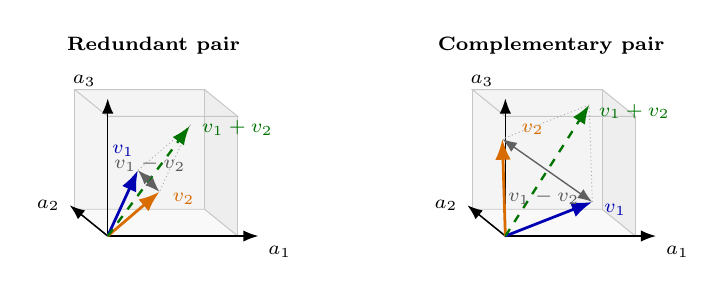
\begin{tikzpicture}[
  font=\scriptsize,
  >=Latex,
  x={(1.65cm,0cm)},
  y={(-0.42cm,0.34cm)},
  z={(0cm,1.52cm)},
  axis3/.style={->, line width=0.55pt},
  cube/.style={line width=0.35pt, gray!45},
  candA/.style={->, line width=1.0pt, blue!70!black},
  candB/.style={->, line width=1.0pt, orange!85!black},
  sumvec/.style={->, dashed, line width=0.85pt, green!45!black},
  guide/.style={densely dotted, line width=0.35pt, gray!65},
  diffline/.style={<->, line width=0.5pt, gray!75!black},
  difflabel/.style={inner sep=0.6pt, gray!70!black},
  vlabel/.style={inner sep=0.6pt}
]

\begin{scope}
\node[font=\bfseries\scriptsize] at (0.48,0.50,1.48) {Redundant pair};
\fill[gray!5] (0,0,0) -- (1,0,0) -- (1,1,0) -- (0,1,0) -- cycle;
\fill[gray!9] (0,1,0) -- (1,1,0) -- (1,1,1) -- (0,1,1) -- cycle;
\fill[gray!13] (1,0,0) -- (1,1,0) -- (1,1,1) -- (1,0,1) -- cycle;
\draw[cube] (0,0,0) -- (1,0,0) -- (1,1,0) -- (0,1,0) -- cycle;
\draw[cube] (0,0,1) -- (1,0,1) -- (1,1,1) -- (0,1,1) -- cycle;
\draw[cube] (0,0,0) -- (0,0,1);
\draw[cube] (1,0,0) -- (1,0,1);
\draw[cube] (0,1,0) -- (0,1,1);
\draw[cube] (1,1,0) -- (1,1,1);
\draw[axis3] (0,0,0) -- (1.16,0,0) node[below right] {\(a_1\)};
\draw[axis3] (0,0,0) -- (0,1.15,0) node[left] {\(a_2\)};
\draw[axis3] (0,0,0) -- (0,0,1.15) node[above left=1pt] {\(a_3\)};
\coordinate (rA) at (0.38,0.58,0.42);
\coordinate (rB) at (0.50,0.40,0.28);
\coordinate (rS) at (0.88,0.98,0.70);
\draw[candA] (0,0,0) -- (rA) node[pos=1.10, above left=2pt, vlabel] {\(v_1\)};
\draw[candB] (0,0,0) -- (rB) node[pos=1.12, below right=2pt, vlabel] {\(v_2\)};
\draw[guide] (rA) -- (rS) -- (rB);
\draw[sumvec] (0,0,0) -- (rS) node[pos=0.98, right=4pt, vlabel] {\(v_1+v_2\)};
\draw[diffline] (rA) -- (rB) node[pos=0.55, left=8pt, above=3pt, difflabel] {\(v_1-v_2\)};
\end{scope}

\begin{scope}[xshift=5.05cm]
\node[font=\bfseries\scriptsize] at (0.48,0.50,1.48) {Complementary pair};
\fill[gray!5] (0,0,0) -- (1,0,0) -- (1,1,0) -- (0,1,0) -- cycle;
\fill[gray!9] (0,1,0) -- (1,1,0) -- (1,1,1) -- (0,1,1) -- cycle;
\fill[gray!13] (1,0,0) -- (1,1,0) -- (1,1,1) -- (1,0,1) -- cycle;
\draw[cube] (0,0,0) -- (1,0,0) -- (1,1,0) -- (0,1,0) -- cycle;
\draw[cube] (0,0,1) -- (1,0,1) -- (1,1,1) -- (0,1,1) -- cycle;
\draw[cube] (0,0,0) -- (0,0,1);
\draw[cube] (1,0,0) -- (1,0,1);
\draw[cube] (0,1,0) -- (0,1,1);
\draw[cube] (1,1,0) -- (1,1,1);
\draw[axis3] (0,0,0) -- (1.16,0,0) node[below right] {\(a_1\)};
\draw[axis3] (0,0,0) -- (0,1.15,0) node[left] {\(a_2\)};
\draw[axis3] (0,0,0) -- (0,0,1.15) node[above left=1pt] {\(a_3\)};
\coordinate (cA) at (0.72,0.20,0.24);
\coordinate (cB) at (0.16,0.72,0.65);
\coordinate (cS) at (0.88,0.92,0.89);
\draw[candA] (0,0,0) -- (cA) node[pos=1.08, below right=1pt, vlabel] {\(v_1\)};
\draw[candB] (0,0,0) -- (cB) node[pos=1.10, right=6pt, vlabel] {\(v_2\)};
\draw[guide] (cA) -- (cS) -- (cB);
\draw[sumvec] (0,0,0) -- (cS) node[pos=0.95, right=4pt, vlabel] {\(v_1+v_2\)};
\draw[diffline] (cA) -- (cB) node[pos=0.54, below=7pt, difflabel] {\(v_1-v_2\)};
\end{scope}
\end{tikzpicture}
}
\caption{Field-aware pair selection as a vector objective. Each axis is a query-field similarity component \(a_i\); actual retrieval vectors are \(m\)-dimensional. A redundant pair concentrates evidence in similar directions, so \(v_1-v_2\) is short. A complementary pair covers different field dimensions, increasing both the joint vector \(v_1+v_2\) and the difference vector \(v_1-v_2\) used by the pair score.}
\label{fig:field-aware-pair-selection}
\end{figure}

Demonstration diversity is not merely topical diversity. Two examples from different domains can still be redundant if both show easy scalar fields and neither illustrates nulls, arrays, or enum decisions. Conversely, two examples from a related family may be complementary if one illustrates absence and empty arrays while the other illustrates populated nested objects and label mapping. Tie-breaking favors stronger individual relevance and stable resource order, but the core decision is pair-level.

\subsection{Prompt Integration}

DRILLER integrates selected examples into the extraction prompt in one of two layouts. The general RAG layout is used when examples are related but not all same-schema matches. Each example is rendered as a self-contained demonstration with its instruction, schema context, source text, and expected output. This gives the model enough context to see how the example output follows from that example's schema before using it analogically.

The same-schema layout is used when all selected examples share the normalized target schema. The shared schema is rendered once, alongside the role instruction, extraction rules, root description when available, and guidance that examples are demonstrations rather than evidence. The examples then omit repeated schema blocks and focus on source-to-output behavior under the common structure. This reduces prompt length and makes contrasting field outcomes more salient.

Pipeline integration depends on the current output interface. In \texttt{Schema-RAG}, examples are rendered in direct final-value form, matching the object shape returned after generation. In \texttt{Reasoned-RAG}, examples are rendered with top-level \texttt{\{reasoning, value\}} objects because the temporary generation interface requires that structure. The reasoning strings demonstrate a local evidence protocol, while the \texttt{value} slots show the values that will later be unwrapped.

\texttt{Mixed-SC} uses the same retrieval machinery inside each trial. Direct trials use the \texttt{Schema-RAG} rendering, and reasoning-augmented trials use the \texttt{Reasoned-RAG} rendering. Each trial performs retrieval independently. Aggregation receives only postprocessed JSON candidates in the final schema shape.

Field-aware retrieval turns the local corpus into an inference-time schema interpretation aid. Same-schema retrieval exploits exact structural matches when available, field-level fallback finds type-compatible analogies, the pair objective favors complementary coverage, and prompt integration adapts examples to the direct, reasoned, and mixed pipelines.

\section{Reasoning-Augmented Extraction}

\texttt{Reasoned-RAG} adds a temporary reasoning interface to the shared extraction pipeline. Some GenSIE fields require local evidence assessment before a value can be produced: the model may need to identify relevant fragments, decide whether evidence is absent, normalize a phrase, or map cues to an enum label. Reasoning-augmented extraction gives each top-level field a structured place for that intermediate decision while preserving the final JSON interface.

In \texttt{Reasoned-RAG}, each top-level field of the target object is temporarily wrapped as an object with two properties:

\begin{verbatim}
{
  "reasoning": "...",
  "value": ...
}
\end{verbatim}

The \texttt{reasoning} property is a string. The \texttt{value} property keeps the original schema of the wrapped field. If the original field is an enum, the \texttt{value} must be one of the enum labels; if it is an array or object, the nested structure remains there; if it is nullable, the \texttt{value} may be JSON \texttt{null} when the schema permits it. The wrapper changes the temporary generation shape, not the semantic target.

The submitted reasoning mode is top-level only. It wraps root object properties, not every nested property recursively. If a top-level field is itself an object or an array of objects, the nested content remains inside \texttt{value} according to the original field schema. This keeps the prompt and response format manageable while asking the model to deliberate at the level of the main requested slots.

The prompt-side effect is a reasoned Pydantic-style schema view. Rather than seeing a top-level field simply as a value of type \(T\), the model sees it as a reasoned value, using the class \texttt{Reasoned[T]}. The extraction instructions ask the model to state what the field requests, identify supporting evidence or absence, and then commit to the final value. This is intended for fields involving nullability, enum classification, boolean inference, normalization, and arrays whose correct value may be empty.

The generation-side effect is equally important. The reasoning interface is part of the strict temporary response schema, so each wrapped top-level field must contain both \texttt{reasoning} and \texttt{value}. This prevents free-form reasoning from leaking outside the JSON object and keeps the final value constrained by the original field type. The wrapper adds a field-local explanation channel without relaxing the schema constraints on the answer.

After generation, postprocessing removes the wrapper. Each top-level object of the form \texttt{\{reasoning, value\}} is replaced by its \texttt{value}; reasoning strings are discarded before the output is returned or passed to self-consistency aggregation. If the expected wrapper structure is malformed and cannot be reliably unwrapped, the extraction record is treated as invalid rather than repaired semantically.

Reasoning-augmented extraction also affects RAG rendering. Examples retrieved for \texttt{Reasoned-RAG} are shown in the same temporary output format expected from the current extractor. A direct example with final field values would be inconsistent with a prompt that asks for top-level \texttt{\{reasoning, value\}} objects. Reasoning-mode examples therefore demonstrate both the evidence protocol and the placement of the final answer in the \texttt{value} slot, while still remaining demonstrations rather than evidence for the current instance.
\section{Postprocessing and Output Normalization}

DRILLER uses deterministic postprocessing to align model outputs with the final schema interface. Even with a strict JSON Schema response format, outputs can contain representation artifacts such as literal Unicode escape strings, the string \texttt{"null"} where JSON \texttt{null} was intended, or temporary reasoning wrappers from \texttt{Reasoned-RAG}. Postprocessing cleans these artifacts.

The first step is JSON parsing. The submitted pipelines expect a JSON object because the prompt asks for JSON only and the request includes a structured response format. If an output cannot be parsed as JSON, the trial is marked invalid rather than repaired by string heuristics. This boundary is especially important for \texttt{Mixed-SC}, where aggregation should combine valid candidate objects rather than fragments of malformed responses.

After parsing, DRILLER applies Unicode cleanup recursively to string values. Spanish text may include diacritics, the letter ñ, inverted punctuation marks, and other characters that can appear inconsistently across model outputs or API layers. The normalizer cleans literal escape artifacts such as \texttt{\textbackslash u00e1} when they appear inside strings and then normalizes strings to Unicode Normalization Form C (NFC). NFC makes visually identical strings more stable for comparison while preserving their textual content.

For \texttt{Reasoned-RAG} and the reasoning-augmented trials of \texttt{Mixed-SC}, postprocessing removes the temporary reasoning/value interface. Each top-level object with \texttt{reasoning} and \texttt{value} fields is replaced by its \texttt{value}. The reasoning text is discarded before the final JSON object is returned and before any self-consistency aggregation is applied. If unwrapping fails because the expected structure is absent or malformed, the trial is invalid.

The prompt asks the model to use JSON \texttt{null} for unsupported information when null is allowed, but models may emit string literals such as \texttt{"null"}, \texttt{"NULL"}, or other casing variants instead. DRILLER converts these string markers to JSON \texttt{null} only at schema positions where \texttt{null} is valid. It does not globally replace all occurrences, because a non-nullable string field should not be silently changed into a null value.

In \texttt{Mixed-SC}, each trial independently performs prompt construction, strict generation, parsing, Unicode cleanup, optional unwrapping, and null coercion. Invalid trials are excluded from aggregation. The aggregator receives postprocessed JSON candidates in the original schema shape; after aggregation, nullable-string coercion may be applied again so selected values remain aligned with schema-valid null representation.

Thus, postprocessing in DRILLER is deterministic, schema-aware, and conservative. It makes generated objects cleaner and compatible with the expected interface while preserving the semantic content produced by the extractor.

\section{Heterogeneous Self-Consistency}

\subsection{Motivation}

Schema-guided extraction can vary across generations even when the output format is constrained. Candidate outputs may differ in whether they include a borderline entity, how they normalize a date, which enum label they choose, or whether they return JSON \texttt{null}. Some of this variance comes from sampling, but some comes from the interface shown to the model. For example, the reasoning-augmented prompt spends more output budget on field-local evidence assessment before committing to values.

In \texttt{Mixed-SC} we use this observation for heterogeneous self-consistency. Rather than sampling one prompt repeatedly, it combines \texttt{Schema-RAG}, which produces final values directly, with \texttt{Reasoned-RAG}, which temporarily produces \texttt{\{reasoning, value\}} objects and then unwraps them. The goal is to obtain candidates with potentially different error patterns. The final decision is not a flat vote over complete JSON strings; it is a recursive schema-aware aggregation over candidate objects.

\subsection{Candidate Generation}

\texttt{Mixed-SC} defines an intended plan of up to four extraction attempts. The plan contains two direct \texttt{Schema-RAG}-style trials and two reasoning-augmented \texttt{Reasoned-RAG}-style trials, ordered as \texttt{Reasoned-RAG}, \texttt{Schema-RAG}, \texttt{Reasoned-RAG}, and \texttt{Schema-RAG}.

The plan is interleaved because execution is budget-aware. If the runner stops early, the available candidate set should not consist only of one extractor family. Interleaving gives the aggregator a chance to see both direct and reasoning-augmented candidates as early as possible, so partial execution still preserves the heterogeneous premise of \texttt{Mixed-SC}. We start with the reasoning-augmented extractor to prioritize the more evidence-sensitive configuration.

Each trial is a complete extraction run. It performs its own RAG retrieval, prompt construction, strict JSON generation, and deterministic postprocessing. Direct trials render examples and schemas in the \texttt{Schema-RAG} format. Reasoning-augmented trials render examples and schemas in the temporary \texttt{Reasoned-RAG} format, so demonstrations contain reasoning/value fields during generation.

Postprocessing is applied before aggregation. Reasoning wrappers are removed, Unicode normalization and schema-aware null coercion are applied, and malformed outputs are rejected. The aggregation stage therefore receives final-shape JSON candidates in the original challenge schema, not raw model messages and not reasoning traces. \texttt{Mixed-SC} aggregates answers, not explanations.

Candidate validity is checked at the trial level. A candidate must parse as JSON and pass required unwrapping. Invalid candidates are excluded from aggregation. If all trials fail to produce valid postprocessed outputs, the system does not fabricate an extraction from partial information.

Trial execution is bounded by an incremental budget planner. Before the first trial, the runner estimates how many planned attempts fit under the effective token and time budgets for the instance. After each completed extraction, it updates the estimate using observed prompt tokens when available, completion tokens, and elapsed trial time, then decides whether another planned extraction can still be attempted. Because the system does not fully control how many tokens a hosted model call will consume, this continuation decision is made after completed trials rather than by assuming that all four planned calls will fit.

\subsection{Schema-Aware Recursive Aggregation}

Aggregation is recursive over the target schema. Complete JSON objects are not treated as indivisible. Instead, DRILLER descends through the schema and combines candidate values according to the expected type at each position. Agreement is measured across trials rather than across raw occurrences alone. This matters because agreement has different meanings for closed labels, free text, nullable fields, nested objects, and arrays.

Clusters are formed using schema-aware similarity. For exact types, including enums, booleans, integers, and numeric values, candidates are grouped by canonical equality. For non-exact types, such as free text and structured array items, candidates are greedily assigned to a compatible cluster only when their schema-aware similarity reaches the active threshold. A cluster's support is the number of distinct trials represented in it. The selected value comes from the cluster with strongest support, with stable occurrence order used as a tie-breaker.

Free-text strings are clustered rather than compared only by byte equality. Candidates may express the same grounded value with minor spelling, accent, punctuation, or phrasing differences. The default string path normalizes text and considers lexical overlap and character n-gram overlap. For a selected non-exact cluster \(C\), the representative is a medoid: the generated candidate \(x \in C\) that maximizes average similarity to the other cluster members, equivalently minimizing average distance:

\[
\operatorname{medoid}(C)=
\arg\max_{x\in C}
\frac{1}{|C|-1}\sum_{y\in C,\,y\ne x}\operatorname{sim}(x,y).
\]

Null values are treated as a separate candidate type. For nullable fields, JSON \texttt{null} is expected when the source text does not support a value. However, null does not win by default in ties: null wins only when its support is strictly greater than the best supported non-null value. This avoids turning uncertainty into absence while still preserving shared abstention when multiple trials independently return null.

Objects are aggregated field by field. For a root object, this allows one candidate to contribute stronger support for one field while another contributes a better-supported value elsewhere. The final object can therefore combine agreement patterns across the candidate set rather than selecting one whole candidate unchanged.

\subsection{Array Aggregation}

Arrays require separate handling because disagreement can involve order, omissions, duplicates, merged items, split items, or outliers. A majority vote over complete arrays would be brittle: two candidates may contain the same substantive items in different orders or differ by one peripheral object. DRILLER therefore aggregates arrays by clustering items across candidate arrays.

The array procedure first collects items from candidate arrays and compares them using schema-aware similarity. For arrays of simple values, item similarity follows the value type. For arrays of objects, object similarity compares corresponding fields with weights influenced by schema type. This allows two object items to align when they refer to the same entity, reaction, ingredient, event, or evidence span even if some attributes differ.

Near-duplicates from the same trial are handled cautiously. A single generated array may repeat one item or produce very similar variants. Such repetitions should not count as independent votes. Before cross-trial clustering, very similar items from the same generated array are deduplicated. During non-exact clustering, the clusterer also tracks trial indexes and prevents a cluster from accepting multiple values from the same trial. Thus support is support by trial: near-duplicates from one verbose array output do not become multiple votes and cannot dominate a cluster by repetition alone.

Arrays of objects may use identity-like fields to improve alignment. Many object-array schemas contain a field that behaves like an identifier: a name, title, mention, text span, ingredient, symptom, reaction, or source fragment. When such a field is detected with sufficient confidence, it guides item matching across trials. Two objects with the same reaction name but different impact labels should be compared as competing descriptions of one item, not as unrelated items. If no useful identity field is detected, the aggregator falls back to broader object similarity.

This alignment is important because object arrays often combine extraction and classification. The identity-like field tells the system which candidate objects correspond; remaining fields can then be compared or aggregated inside that item cluster. Imperfect identity detection is also a risk: a generic attribute may align unrelated objects, while failure to detect an identity field may split corresponding objects into duplicate clusters.

\subsection{Recall-Biased Selection}

After clustering array items, the aggregator selects a final array. The submitted design builds candidate final arrays from item clusters, including support-threshold arrays and a greedy MBR-style candidate. MBR stands for minimum Bayes risk: in this context, choosing the candidate final array that minimizes expected disagreement, or loss, against the observed candidate arrays.

Candidate arrays are scored by agreement with the observed arrays under schema-aware item similarity rather than exact positional equality. This allows two arrays to agree strongly even when the same substantive items appear in different orders, or when object items differ only in secondary fields.

Selection is recall-biased when candidate arrays have similar scores. Among arrays within a tolerance of the best score, the selector prefers the longer array, then the higher-scoring one, then the earlier candidate. This favors retaining supported items when evidence from trials is close. The longer array is not accepted unconditionally; it must remain competitive under the consensus objective.

The design trades omission against over-extraction. A stricter selector would discard more borderline items, improving precision in some cases but risking missed entities or list elements. DRILLER's recall-biased selector keeps items with enough support to remain near the best consensus score, which is useful for unordered lists, object arrays, and evidence collections where candidates often agree on a core set but vary on peripheral supported items.

\subsection{Conservativeness and Failure Modes}

Aggregation is conservative in that it selects among generated candidates rather than inventing semantic content. Exact scalar types are selected by canonical equality groups; non-exact string clusters choose a generated representative; arrays are built from generated item clusters. The aggregator does not use external knowledge, synthesize new enum labels, or create facts absent from all candidate outputs.

Self-consistency is still not a guarantee of correctness. If multiple trials share the same misunderstanding of a field description, attend to the same distractor mention, or overtrust an unsupported fact, aggregation can preserve that mistake with high support. Heterogeneous prompting reduces reliance on one prompt representation, but all trials still share the source text, target schema, local FSP corpus, model endpoint, and broad extraction rules.

Array aggregation has additional failure modes. The recall-biased selector may retain extra borderline items, and identity-field detection can misalign object items or fail to merge true matches. These risks are the cost of trying to preserve recall in schemas where missing list members are common and where item order is not meaningful.

\texttt{Mixed-SC} also increases inference cost. It requests up to four model calls rather than one, and up to two calls use reasoning-augmented generation, which can produce longer intermediate outputs before unwrapping.

\section{Experimental Setup}

The submitted solution consists of three final pipelines: \texttt{Schema-RAG}, \texttt{Reasoned-RAG}, and \texttt{Mixed-SC}. These correspond to the submitted names \path{enriched-schema-rag}, \path{enriched-inline-reasoning-rag}, and \path{mixed-extractors-self-consistency-rag}. We also report a non-RAG baseline for comparison.

The results below are computed from our final test-set run logs rather than from an official leaderboard release. They cover 145 test instances evaluated with two hosted models exposed through an OpenAI-style chat interface: \path{google_gemma-4-e4b-it} and \path{qwen/qwen3-14b}. Baseline, \texttt{Schema-RAG}, and \texttt{Mixed-SC} were run with both models; the available \texttt{Reasoned-RAG} run uses Gemma only. The GenSIE overview paper remains the authoritative source for dataset construction, official ranking, model selection, and shared-task scoring details \cite{gensie2026overview}.

We report micro-averaged precision, recall, and \(F_1\) by summing the evaluator's true-positive mass, gold keys, and system keys over a subset before computing the metric. Token counts are the average total input-plus-output tokens per instance from the run logs. We do not report wall-clock-time comparisons: the logs do not provide enough granular traceability to separate our code from hosted backend latency and small-language-model generation delays inside the evaluation service. We also report \texttt{calls=0}, the number of instances for which no model call was completed; these cases contribute no true positives and explain much of the gap between all-instance and nonzero-call analyses.

The test set contains 23 unique schema fingerprints under the same structural normalization used by retrieval. Ten fingerprints are present in the development/FSP corpus, but they account for only 36 of 145 test instances. The remaining 13 unseen fingerprints account for 109 instances. Before the test set was released, the task description suggested a roughly balanced mixture of seen and unseen schemas; this influenced the design toward supporting both exact same-schema reuse and complementary field-level fallback. The final test distribution is more skewed toward unseen-schema instances, making the fallback route more central than expected.

\section{Results and Analysis}

Table~\ref{tab:main-results} shows the aggregate runs. Since the two models have different baselines, raw \(F_1\) is not by itself a representative cross-model comparison. We therefore also report the fraction of the baseline-to-1.0 \(F_1\) gap closed by each non-baseline run, \((F_1^{system}-F_1^{baseline})/(1-F_1^{baseline})\), computed within the same model. Accordingly, the analysis emphasizes gap closed relative to each model's baseline rather than absolute \(F_1\) alone. For both models, \texttt{Schema-RAG} closes a substantial part of the baseline gap. With Gemma, \texttt{Schema-RAG} obtains the highest aggregate \(F_1\) among the available Gemma runs, while \texttt{Reasoned-RAG} is close but slightly lower. With Qwen, \texttt{Mixed-SC} gives the best aggregate \(F_1\), narrowly ahead of \texttt{Schema-RAG}, but at much higher token cost.

\begin{table}[!htbp]
\centering
\caption{Test-set metrics from final run logs. Tokens are average total tokens per instance. Gap is the fraction of the model-specific baseline-to-1.0 \(F_1\) gap closed.}
\label{tab:main-results}
\scriptsize
\begin{tabular}{@{}llrrrrrr@{}}
\toprule
Model & Pipeline & Prec. & Rec. & \(F_1\) & Gap & Tok. & \texttt{calls=0} \\
\midrule
Gemma & Baseline & 0.702 & 0.639 & 0.669 & -- & 3691 & 18 \\
Gemma & \texttt{Schema-RAG} & 0.805 & 0.699 & 0.748 & 23.9\% & 4904 & 18 \\
Gemma & \texttt{Reasoned-RAG} & 0.807 & 0.691 & 0.744 & 22.8\% & 8137 & 18 \\
Gemma & \texttt{Mixed-SC} & 0.807 & 0.689 & 0.743 & 22.4\% & 13670 & 20 \\
\midrule
Qwen & Baseline & 0.699 & 0.590 & 0.640 & -- & 3671 & 18 \\
Qwen & \texttt{Schema-RAG} & 0.793 & 0.683 & 0.734 & 26.1\% & 5047 & 20 \\
Qwen & \texttt{Mixed-SC} & 0.800 & 0.702 & 0.747 & 29.8\% & 12688 & 18 \\
\bottomrule
\end{tabular}
\end{table}

Figure~\ref{fig:main-result-bars} visualizes the same aggregate results. The left panel emphasizes the baseline-normalized view: \texttt{Schema-RAG} closes a similar fraction of the available gap for both models, while Qwen \texttt{Mixed-SC} closes the largest fraction but with the token cost shown in Table~\ref{tab:main-results}. The right panel keeps the raw precision, recall, and \(F_1\) values visible for each model-pipeline pair.

\begin{figure}[!htbp]
\centering
\begin{minipage}[t]{0.44\linewidth}
\centering
\begin{tikzpicture}
\begin{axis}[
  ybar,
  width=\linewidth,
  height=0.22\textheight,
  ymin=0,
  ymax=34,
  ylabel={Gap closed (\%)},
  symbolic x coords={S-RAG,R-RAG,Mixed-SC},
  xtick=data,
  xticklabel style={font=\scriptsize},
  yticklabel style={font=\scriptsize},
  label style={font=\scriptsize},
  legend style={
    font=\scriptsize,
    at={(0.5,1.03)},
    anchor=south,
    legend columns=2,
    draw=none
  },
  bar width=8pt,
  enlarge x limits=0.28,
  nodes near coords,
  nodes near coords style={font=\tiny},
  every node near coord/.append style={
    /pgf/number format/fixed,
    /pgf/number format/precision=1
  }
]
\addplot coordinates {(S-RAG,23.9) (R-RAG,22.8) (Mixed-SC,22.4)};
\addplot coordinates {(S-RAG,26.1) (Mixed-SC,29.8)};
\legend{Gemma,Qwen}
\end{axis}
\end{tikzpicture}
\end{minipage}\hfill
\begin{minipage}[t]{0.53\linewidth}
\centering
\begin{tikzpicture}
\begin{axis}[
  xbar,
  width=\linewidth,
  height=0.22\textheight,
  xmin=0.55,
  xmax=0.84,
  xlabel={Score},
  symbolic y coords={Q-MSC,Q-SR,Q-B,G-MSC,G-RR,G-SR,G-B},
  ytick=data,
  yticklabel style={font=\tiny},
  xticklabel style={font=\tiny},
  label style={font=\scriptsize},
  legend style={
    font=\tiny,
    at={(0.5,1.03)},
    anchor=south,
    legend columns=3,
    draw=none
  },
  bar width=2.2pt,
  enlarge y limits=0.12
]
\addplot coordinates {
  (0.702,G-B) (0.805,G-SR) (0.807,G-RR) (0.807,G-MSC)
  (0.699,Q-B) (0.793,Q-SR) (0.800,Q-MSC)
};
\addplot coordinates {
  (0.639,G-B) (0.699,G-SR) (0.691,G-RR) (0.689,G-MSC)
  (0.590,Q-B) (0.683,Q-SR) (0.702,Q-MSC)
};
\addplot coordinates {
  (0.669,G-B) (0.748,G-SR) (0.744,G-RR) (0.743,G-MSC)
  (0.640,Q-B) (0.734,Q-SR) (0.747,Q-MSC)
};
\legend{Prec.,Rec.,\(F_1\)}
\end{axis}
\end{tikzpicture}
\end{minipage}
\caption{Aggregate result views. Left: fraction of model-specific baseline \(F_1\) gap closed by each non-baseline run. Right: precision, recall, and \(F_1\) by model-pipeline pair. Abbreviations: G/Q = Gemma/Qwen, B = baseline, SR = \texttt{Schema-RAG}, RR = \texttt{Reasoned-RAG}, MSC = \texttt{Mixed-SC}. Qwen \texttt{Reasoned-RAG} was not available.}
\label{fig:main-result-bars}
\end{figure}

\subsection{Retrieval Contribution}

The comparison with the baseline is the clearest available evidence for the usefulness of retrieval, although it is not a controlled ablation of every prompt change. As Table~\ref{tab:component-deltas} shows, \texttt{Schema-RAG} improves \(F_1\) by 0.079 with Gemma and 0.094 with Qwen on all instances, closing 23.9\% and 26.1\% of the respective baseline gaps. When instances with zero calls on either side are removed, the gains increase to 0.094 and 0.119, closing 33.7\% and 38.2\% of the nonzero-call baseline gaps.

\begin{table}[!htbp]
\centering
\caption{Selected component comparisons. ``No zero calls'' excludes instances where either compared run has \texttt{calls=0}. Token deltas are average total tokens per instance. Gap columns are shown only for comparisons against the model-specific baseline.}
\label{tab:component-deltas}
\scriptsize
\begin{tabularx}{\linewidth}{@{}>{\raggedright\arraybackslash}Xrrrrr@{}}
\toprule
Comparison & \(\Delta F_1\) & Gap & No-zero \(\Delta F_1\) & No-zero gap & \(\Delta\) tok. \\
\midrule
Gemma: \texttt{Schema-RAG} vs. baseline & +0.079 & 23.9\% & +0.094 & 33.7\% & +1213 \\
Qwen: \texttt{Schema-RAG} vs. baseline & +0.094 & 26.1\% & +0.119 & 38.2\% & +1376 \\
Gemma: \texttt{Mixed-SC} vs. \texttt{Schema-RAG} & -0.005 & -- & +0.004 & -- & +8766 \\
Qwen: \texttt{Mixed-SC} vs. \texttt{Schema-RAG} & +0.013 & -- & +0.006 & -- & +7641 \\
\bottomrule
\end{tabularx}
\end{table}

The retrieval-only replay selected the same-schema route for 36 instances and attempted the field-aware fallback for the remaining 109. Ten fallback instances enter a retrieval-failure path, so the route-level field-RAG comparison below uses the 99 instances with complete field-embedding diagnostics. This split aligns with the seen/unseen schema split under the structural fingerprint.

\begin{table}[!htbp]
\centering
\caption{Performance by retrieval route. Same-schema contains 36 instances; Field-RAG contains the 99 fallback instances with complete field-embedding diagnostics.}
\label{tab:route-performance}
\scriptsize
\begin{tabular}{@{}llrrrrrr@{}}
\toprule
& & \multicolumn{3}{c}{Same-schema} & \multicolumn{3}{c}{Field-RAG} \\
\cmidrule(lr){3-5}\cmidrule(l){6-8}
Model & Pipeline & Prec. & Rec. & \(F_1\) & Prec. & Rec. & \(F_1\) \\
\midrule
Gemma & Baseline & 0.639 & 0.667 & 0.653 & 0.725 & 0.693 & 0.709 \\
Gemma & \texttt{Schema-RAG} & 0.765 & 0.737 & 0.751 & 0.830 & 0.756 & 0.791 \\
Gemma & \texttt{Reasoned-RAG} & 0.804 & 0.775 & 0.789 & 0.820 & 0.731 & 0.773 \\
Gemma & \texttt{Mixed-SC} & 0.801 & 0.742 & 0.770 & 0.821 & 0.739 & 0.778 \\
\midrule
Qwen & Baseline & 0.622 & 0.558 & 0.588 & 0.725 & 0.660 & 0.691 \\
Qwen & \texttt{Schema-RAG} & 0.734 & 0.707 & 0.720 & 0.825 & 0.743 & 0.782 \\
Qwen & \texttt{Mixed-SC} & 0.779 & 0.779 & 0.779 & 0.818 & 0.745 & 0.780 \\
\bottomrule
\end{tabular}
\end{table}

\texttt{Schema-RAG} improves over baseline in both routes: with Gemma, \(F_1\) increases by 0.098 on same-schema instances and 0.082 on field-RAG instances; with Qwen, the corresponding gains are 0.132 and 0.091. Figure~\ref{fig:rag-route-delta} shows that same-schema reuse is helpful, but not the only source of gains. Excluding zero-call instances, the field-RAG gains are 0.092 for Gemma and 0.107 for Qwen. These results suggest that retrieval is not only exploiting exact schema reuse; complementary field-level examples also contribute on unseen schemas when the field-aware route completes. Additional retrieval diagnostics are summarized in Appendix~\ref{sec:appendix-retrieval-diagnostics}.

\begin{figure}[!htbp]
\centering
\begin{tikzpicture}
\begin{axis}[
  ybar,
  width=0.58\linewidth,
  height=0.22\textheight,
  ymin=0,
  ymax=0.15,
  ylabel={\(\Delta F_1\) vs. baseline},
  symbolic x coords={Same-schema,Field-RAG},
  xtick=data,
  xticklabel style={font=\scriptsize},
  yticklabel style={font=\scriptsize},
  label style={font=\scriptsize},
  legend style={
    font=\scriptsize,
    at={(0.5,1.03)},
    anchor=south,
    legend columns=2,
    draw=none
  },
  bar width=10pt,
  enlarge x limits=0.35,
  nodes near coords,
  nodes near coords style={font=\tiny},
  every node near coord/.append style={
    /pgf/number format/fixed,
    /pgf/number format/precision=3
  }
]
\addplot coordinates {(Same-schema,0.098) (Field-RAG,0.082)};
\addplot coordinates {(Same-schema,0.132) (Field-RAG,0.091)};
\legend{Gemma,Qwen}
\end{axis}
\end{tikzpicture}
\caption{\texttt{Schema-RAG} \(F_1\) gain over the baseline by retrieval route. Field-RAG includes the 99 fallback instances with complete field-embedding diagnostics.}
\label{fig:rag-route-delta}
\end{figure}

\subsection{Reasoning and Self-Consistency}

\texttt{Reasoned-RAG} was available only for Gemma. Its aggregate \(F_1\) is slightly below \texttt{Schema-RAG} (0.744 vs. 0.748), closes 22.8\% of the baseline gap compared with 23.9\% for \texttt{Schema-RAG}, and uses substantially more tokens. The route-level pattern is mixed: relative to \texttt{Schema-RAG}, reasoning improves the same-schema subset by 0.039 \(F_1\) but is lower by 0.018 on field-RAG instances. A plausible interpretation is that explicit top-level evidence wrappers help when retrieved examples share the exact output contract, but add overhead when the examples are only field-complementary. This should be treated as a diagnostic observation rather than a causal result, because Qwen reasoning runs and controlled reasoning ablations are not yet available.

\texttt{Mixed-SC} does not consistently outperform the strongest single-call extractor. For Gemma it is slightly below \texttt{Schema-RAG} on all instances and only marginally above it after zero-call instances are excluded. For Qwen it improves the aggregate \(F_1\) by 0.013, increasing the gap closed from 26.1\% to 29.8\%, but the nonzero-call gain is only 0.006. The cost is much larger: \texttt{Mixed-SC} adds roughly 7.6K--8.8K average tokens per instance over \texttt{Schema-RAG}. Its main benefit appears in same-schema subsets, where it improves over \texttt{Schema-RAG} by 0.020 with Gemma and 0.059 with Qwen, while it is flat or lower on field-RAG subsets. This supports using self-consistency as a robustness mechanism, but not as a uniformly efficient default.

\subsection{Failure Patterns}

The largest non-semantic failure mode is zero completed model calls. Eighteen such instances are common across the main runs: 10 \texttt{TaxonomicClassification} instances and 8 \texttt{ClinicalTrialRecord} instances. The former coincide with the retrieval-failure path in our replay, while the latter pass retrieval and fail later in execution. A few extra zero-call cases are run-specific, including two in Gemma \texttt{Mixed-SC} and two in Qwen \texttt{Schema-RAG}. Because these failures dominate some schema and route subsets, we report both all-instance metrics and nonzero-call comparisons.

Among successful calls, the systems usually produce fewer keys than the gold output on average. \texttt{Schema-RAG} reduces this gap relative to the baseline in several subsets, but underproduction remains visible in the aggregate. This is consistent with the task's strict grounding requirement: omitting uncertain fields tends to raise precision relative to recall, while array and object fields can lose multiple gold keys when a list item or nested object is missed. A field-level error analysis requires aligned prediction details and is left for future controlled analysis.

We keep several exploratory diagnostics out of the main paper body to avoid overinterpreting non-controlled correlations: per-domain and per-schema tables, selected-example hub analyses, pair-score and coverage tertiles, task-level improvement/regression lists, and wall-clock-time comparisons. The appendix retains only the retrieval diagnostics needed to support the main same-schema versus field-RAG interpretation.

\section{Limitations}

DRILLER is designed for schema-variable extraction, and several limitations follow from that design. The first is dependence on a local few-shot prompting corpus. The demonstrations are synthetic and curated, which gives controlled coverage of nulls, populated values, enum choices, arrays, nested structures, and distractors, but also requires careful construction and review. Each case must keep the instruction, source text, schema, output, and rationale mutually consistent. Errors or narrow coverage in the corpus can propagate into prompts.

Coverage remains incomplete because GenSIE schemas vary by instance. A demonstration family can represent one schema well while failing to cover later fields with different names, descriptions, nesting, or value regimes. Complementary examples reduce reliance on one output pattern, but they cannot guarantee that every private evaluation schema has a close analogue. If retrieved examples mostly show populated arrays, frequent enum labels, or non-null values, they may still bias the model toward overproduction.

Retrieval depends on schema information quality. Same-schema retrieval is useful when structurally matching examples exist, but it has limited value when the local corpus lacks the target schema. Field-level fallback is more flexible, yet it relies on names, descriptions, type representations, and coarse type classes. Sparse or generic descriptions can make unrelated fields appear similar, while equivalent fields with different wording can be missed. Type compatibility prevents many implausible alignments, but it can also exclude examples whose meanings are related despite different schema forms.

The reasoning/value wrapper in \texttt{Reasoned-RAG} is a cost trade-off. It can encourage explicit evidence assessment and clearer decisions between a value and \texttt{null}, but it increases output length, consumes context, and may raise latency or token cost. Because the submitted wrapper is top-level only, it does not give every nested field its own explicit evidence scaffold. This keeps the temporary schema manageable, but complex nested objects may still require decisions that are only indirectly guided by top-level reasoning.

\texttt{Mixed-SC} further increases inference cost by requesting up to four trials, including up to two reasoning-augmented calls. Runtime budgets may limit completed trials, and practical efficiency depends on the model, backend, decoding configuration, and official token accounting. Its value must therefore be judged jointly by extraction quality and cost.

Aggregation is heuristic. It votes over closed scalar values, clusters strings, aggregates objects field by field, clusters array items, and selects arrays with a recall-biased strategy. These rules are schema-aware and conservative in the sense that selected representatives come from generated candidates, but they are not optimality guarantees. Shared mistakes can be reinforced, borderline array items can be retained, and imperfect identity-field detection can misalign object arrays.

Finally, component-level effects remain empirical questions. The paper describes the submitted architecture, but claims about the separate impact of schema rendering, retrieval, same-schema prompting, reasoning wrappers, postprocessing, or heterogeneous self-consistency require controlled ablations. Results may also depend strongly on the hosted model's structured-output behavior, context limits, multilingual extraction ability, and instruction following.

\section{Conclusion}

DRILLER submitted a modular schema-guided extraction system for GenSIE 2026. The system treats each instance as Spanish information extraction under a variable JSON Schema, where the central challenge is interpreting field semantics from the current instruction, schema, and source text while returning grounded schema-conformant JSON.

The three submitted pipelines are \texttt{Schema-RAG}, \texttt{Reasoned-RAG}, and \texttt{Mixed-SC}. All use retrieval-augmented prompting. The common extraction spine combines schema-readable Pydantic-style prompting, strict structured JSON generation, field-aware few-shot retrieval, and conservative postprocessing. \texttt{Reasoned-RAG} adds temporary top-level reasoning/value wrappers that are removed before final output. \texttt{Mixed-SC} combines direct and reasoning-augmented candidates through heterogeneous self-consistency and recursive schema-aware aggregation.

The main design principle is to treat the schema as a runtime semantic specification rather than only an output validator. Readable prompt schemas help the model interpret fields; strict generation constrains the response interface; retrieved examples illustrate field behavior; postprocessing normalizes representation-level artifacts without semantic repair; and aggregation reconciles candidate values according to schema type.

Future work should strengthen both retrieval and aggregation. Learned retrieval could complement schema fingerprints and field-similarity heuristics, especially when field descriptions are sparse. Automatic validation of FSP cases would help detect inconsistent demonstrations before they enter prompts. Aggregation could benefit from better uncertainty estimates, learned item alignment, and schema-specific constraints. Controlled ablations are needed to measure component contributions, and robust array/object extraction remains a priority because omissions, duplicates, and field-alignment errors interact most strongly in nested structures.

\section*{Declaration on Generative AI}

During the preparation of this manuscript, generative AI tools were used to assist with repository inspection, organization of technical notes, drafting, and language editing. The authors reviewed, edited, and approved the final content and take full responsibility for the submitted paper. The DRILLER system also uses synthetic and curated few-shot resources as part of its retrieval component; any generative assistance involved in preparing those resources was followed by manual review and validation.

% TODO: Verify whether IberLEF/CEUR requires a specific official wording for this declaration.


\bibliography{references}

\end{document}
